% se puede agregar la opción [english] para 
%  memorias o tesis en inglés (borrando el archivo .aux)
\documentclass[hyphens]{umemoria} 
%\includeonly{teorico}
\depto{Departamento de Física}
\author{Diego Antonio Román Cortés}
\title{Redes multiorbitales basadas en moléculas fotónicas}

% incluir ambos comandos para una doble titulación
%  o quitar el comando que no aplica
%\memoria{Ingenier[o/a?] Civil en ???}
\tesis{Magíster en Ciencias, mención en Física}
%\tesis{Doctor en ???} % incluir solo este comando para doctorados

% puede haber varios profesores guía seperados por coma;
% pero si es una memoria, solo puede haber un profesor guía
\guia{Rodrigo Andrés Vicencio Poblete} 

% puede haber varios profesores co-guía seperados por coma;
% pero si es una memoria, el profesor co-guía será el primer
% integrante de la comisión
%\coguia{Nombre Completo Co-Guía} % incluir en caso de co-guía de *tesis*

%\cotutela{Nombre Institución} % incluir en caso de cotutela

\comision{Jaime Anguita García, Pedro Orellana}

\auspicio{los proyectos Instituto Milenio para la Investigación en Óptica (MIRO) ICN17$\_$012 y Fondecyt Regular 1231313 \\ Powered@NLHPC: Esta tesis fue parcialmente apoyada por la infraestructura de supercómputo del NLHPC (CCSS210001)} % incluir en caso de recibir financiamiento

% tiene que ser el año en que se da el examen de título/grado (defensa)
%\anho{2021} % incluir solo para reemplazar el año actual

\usepackage{amsmath}
\usepackage{bm}
\usepackage{lipsum}
\usepackage{pgfplots}
\usepackage{txfonts}
\usepackage{graphicx}
%\usepackage[spanish, es-nodecimaldot]{babel}
\usepackage{float}
\usepackage[figurename=Figura]{caption}
\usepackage[numbers, sort&compress]{natbib}
%\usepackage[hyphens]{url}
\usepackage{indentfirst}
\usepackage{hyperref}
\usepackage{xcolor}
\usepackage{ragged2e}
\usepackage{cancel}
\usepackage[rightcaption]{sidecap}
\usepackage{titlesec}
\begin{document}

\frontmatter
\maketitle

\begin{resumen}

\end{resumen}

% opcional: incluir para tesis en inglés;
%  en este caso hay que tener el resumen y abstract
%   en ambos idiomas
%\begin{abstract}
%\lipsum[1-4]
%\end{abstract}

\begin{dedicatoria}


Mas si buscáis descubrimientos\\
Tierras irrealizables más allá de los cielos\\
Vegetante obsesión de musical congoja\\
Volvamos al silencio\\

Trampas de luz y cascadas lujosas\\
Trampas de perla y de lámpara acuática\\
Anda como los ciegos con sus ojos de piedra\\
Presintiendo el abismo a todo paso\\
Mas no temas de mí que mi lenguaje es otro\\
No trato de hacer feliz ni desgraciado a nadie\\
Ni descolgar banderas de los pechos\\
Ni dar anillos de planetas\\
Ni hacer satélites de mármol en torno a un talismán ajeno\\
Quiero darte una música de espíritu\\
Música mía de esta cítara plantada en mi cuerpo\\
Música que hace pensar en el crecimiento de los árboles\\
Y estalla en luminarias dentro del sueño\\
\textnormal{\\Altazor, Vicente Huidobro}
\end{dedicatoria}

\begin{thanks}

\end{thanks}

\tableofcontents
%\listoftables % opcional
\listoffigures % opcional

\mainmatter
\titleformat{\chapter}
  {\normalfont\LARGE\bfseries}{\thechapter.}{1em}{}
\titlespacing*{\chapter}{0pt}{3.5ex plus 1ex minus .2ex}{2.3ex plus .2ex}

\chapter{Introducción}

Durante la última década, varios Premios Nobel en Física han estado estrechamente ligados a la óptica \cite{nobel}: por la generación de pulsos ultracortos de luz —femtosegundos \cite{femto1} y luego attosegundos \cite{atto1, atto2, atto3}—, por experimentos pioneros con fotones entrelazados \cite{photons1, photons2, photons3}, por el desarrollo de pinzas ópticas \cite{opticaltweezers} y por la invención de LEDs de alta eficiencia \cite{led1, led2, led3}. Estos avances fundamentales han impulsado aplicaciones industriales, biomédicas, en telecomunicaciones e incluso en defensa. Una aplicación cotidiana destacada es la fibra óptica, que actúa como guía de onda para la luz y constituye hoy el principal medio de transmisión de datos a nivel global \cite{fibra2, fibra}.

Muchos de estos desarrollos se han visto potenciados por la técnica de \textit{escritura láser de femtosegundos}, que permite fabricar redes fotónicas tridimensionales de guías de onda con precisión micrométrica. Esta tecnología ha habilitado la realización experimental de redes con geometrías complejas y grados de libertad artificiales, y ha sido utilizada para estudiar fenómenos como oscilaciones de Bloch \cite{BlochOsci}, localización de Anderson \cite{Anderson}, dinámica de bandas planas \cite{lieb1, lieb2, artificialFB, FBdynamics}, fases topológicas \cite{obstopo, obsfloquet, topo1dphoto, toporusos}, formación de solitones no lineales \cite{discretesolitons} e incluso la propagación de luz cuántica \cite{qed, squeezed, topoquantum}.

Dentro de este marco, el presente trabajo se enfoca en el estudio de redes fotónicas \textit{multiorbitales}, en las que los modos transversales de la luz —en particular los modos \( P \), de simetría antisimétrica— actúan como grados de libertad internos que pueden aprovecharse para enriquecer la dinámica óptica. A diferencia de los sistemas convencionales, donde se propaga solamente el modo fundamental (\( S \)), las redes multiorbitales permiten emular estructuras más complejas, como acoplamientos interorbitales o interferencias moduladas por la geometría.

Uno de los fenómenos experimentales que motiva este estudio es el \textit{ángulo de invisibilidad} \cite{Pmodecoupling}, descrito en el Capítulo~\ref{cap:invisibility}. En ciertas condiciones geométricas, los modos \( P \) se desacoplan completamente unos de otros, permaneciendo ópticamente \textit{invisibles}. Este fenómeno pone de manifiesto que la simetría transversal de los modos no solo es relevante, sino que puede ser usada activamente como herramienta de control. Este principio guía la exploración de nuevas formas de localización, filtrado y direccionamiento de luz en dispositivos fotónicos integrados.

Luego, se utiliza el concepto de \textit{acoplamiento interorbital SP}, un mecanismo que permite hibridar modos \( S \) y \( P \) ajustando finamente sus constantes de propagación a través del control de la potencia del láser de escritura \cite{interorbital}. Este acoplamiento da lugar a una dinámica rica, especialmente cuando se implementa en redes periódicas.

En el Capítulo~\ref{cap:molecules}, este principio se aplica a la construcción de moléculas fotónicas —pares de guías fuertemente acopladas— cuyas combinaciones simétrica y antisimétrica funcionan como orbitales efectivos. Sobre esta base, se implementa experimentalmente el modelo \textit{SP-SSH} \cite{SPSSH}, una extensión multiorbital del modelo de Su-Schrieffer-Heeger \citep{ssh}. Este sistema presenta una \textit{doble transición de fase topológica}, determinada por dos parámetros independientes: la dimerización geométrica y el desintonizado de las constantes de propagación entre los $S$ y $P$. La existencia de tres fases distintas —con dos, cuatro o ningún modo de borde— se analiza mediante la polarización de bulto y técnicas espectrales.

Ambas líneas —la invisibilidad angular y el acoplamiento SP— se articulan bajo una visión común: aprovechar la \textit{estructura geométrica de los modos guiados} como un nuevo recurso físico en fotónica.

\vspace{1em}

Este trabajo se organiza de la siguiente manera:

El Capítulo~\ref{cap:teo} introduce el formalismo teórico utilizado a lo largo de la tesis, incluyendo los principios de propagación modal, acoplamiento en redes discretas y conceptos topológicos asociados a bandas ópticas.

En el Capítulo~\ref{cap:num} se presentan las herramientas numéricas utilizadas. Se describe el método de Expansión en Modos Normales (EME), que permite estudiar el comportamiento estacionario de la luz, junto con otras metodologías como el método de propagación de haces (BPM) y la teoría de modos acoplados (CMT).

El Capítulo~\ref{cap:exp} detalla la técnica experimental de escritura láser, con énfasis en los parámetros relevantes para diseñar redes multiorbitales tridimensionales.

En el Capítulo~\ref{cap:invisibility} se estudia el fenómeno de invisibilidad modal de los modos \( P \), caracterizando experimentalmente la geometría crítica que conduce al desacoplamiento óptico de estos modos. Esta propiedad se pone a prueba en una red tipo panal de abeja. Para lograr una concordancia cuantitativa entre la teoría y el experimento, se introduce un modelo extendido que incorpora tanto la \textit{no ortogonalidad} entre los modos como \textit{acoplamientos de largo alcance} entre guías no adyacentes.

El Capítulo~\ref{cap:molecules} analiza la formación de moléculas fotónicas y la ingeniería de sus modos internos. A partir de estas, se implementa y caracteriza una red SP-SSH, incluyendo el estudio de sus fases topológicas mediante simulaciones y análisis espectrales.

Finalmente, el Capítulo~\ref{cap:conclu} presenta las conclusiones del trabajo y discute posibles extensiones hacia otras plataformas fotónicas.




\chapter{Marco teórico}

\section{Desde las ecuaciones de Maxwell a propagación de la luz en guías de onda dieléctricas}

Esta tesis estudia el comportamiento de luz láser de baja potencia (1 mW de potencia de salida) propagada en guías de onda dieléctricas escritas dentro de una muestra de borosilicato. Es por ello que se supone un medio lineal no magnético libre de fuentes de carga y de corriente. Las ecuaciones de Maxwell (SI) en este régimen son:
\begin{align}
	\nabla\cdot\textbf{D} &= 0, \label{eqn:gauss}
	\\	
	\nabla\times\textbf{E} &= -\frac{\partial \textbf{B}}{\partial t}, \label{eqn:faraday-lenz}
	\\	
	\nabla\cdot\textbf{B} &= 0, \label{eqn:div0}
	\\	
	\nabla\times\textbf{H} &= \frac{\partial \textbf{D}}{\partial t}, \label{eqn:ampere-maxwell}
\end{align}
donde \textbf{E}, \textbf{B}, $\textbf{D}=\varepsilon(\textbf{r})\textbf{E}$ y $\textbf{H}=\textbf{B}/\mu_0$ son los campos eléctrico, campo de densidad de flujo magnético, campo desplazamiento eléctrico y campo magnético, respectivamente. Las guías de onda son invariantes en la dirección de propagación $z$, por lo que el índice de refracción $n=\sqrt{\varepsilon/\varepsilon_0}$ dependerá de las coordenadas transversales al eje óptico, es decir, $n \equiv n(x,y) = n_0 + \Delta n(x,y)$, con $n_0=1.47$ el índice de refracción del borosilicato y $\Delta n \sim 10^{-5}-10^{-3}$ el contraste de las guías de onda.

Aplicando rotor por la izquierda a la ecuación de Faraday-Lenz (\ref{eqn:faraday-lenz}), usando la ecuación de Ampère-Maxwell (\ref{eqn:ampere-maxwell}) y asumiendo una solución temporal harmónica proporcional a $e^{-i\omega t}$ se tiene:

\begin{align}
	\nabla\times\nabla\times\textbf{E} &= -\frac{\partial}{\partial t}(\nabla\times\textbf{B}) = -\frac{\partial}{\partial t}\left(\mu_0\frac{\partial \textbf{D}}{\partial t}\right) = -\frac{n^2}{c^2}\frac{\partial^2 \textbf{E}}{\partial t^2} = n^2k_0^2 \textbf{E}, \label{eqn:rotordoble}
\end{align}
donde $k_0 \equiv \omega/c$ es el número de onda en el vacío. Notemos que, por identidad de cálculo vectorial, se tiene que $\nabla\times\nabla\times\textbf{E} = \nabla(\nabla\cdot\textbf{E}) - \nabla^2\textbf{E}$, y usando la ley de Gauss (\ref{eqn:gauss}) se deduce que $\nabla\cdot \textbf{E} = -\nabla(n^2)\cdot\textbf{E}/n^2$.

Con esto, se obtiene la ecuación 

\begin{equation}
	(\nabla^2  + k_0^2n^2)\textbf{E} = -\nabla\left( \frac{\nabla n^2}{n^2} \cdot \textbf{E}  \right). \label{eqn:helmholz}
\end{equation}

Análogamente para \textbf{H}, es posible aplicar rotor a la ecuación de Ampère-Maxwell (\ref{eqn:ampere-maxwell}) y usar la ecuación de Faraday-Lenz (\ref{eqn:faraday-lenz}) en conjunto con la divergencia nula de \textbf{B} (\ref{eqn:div0}) y por consiguiente de \textbf{H}:

\begin{align}
	\nabla\times\nabla\times \textbf{H} &= -i \omega \nabla\times\left(\epsilon_0 n^2 \textbf{E}\right) = -i\omega \left(n^2 \nabla\times \textbf{E} + \nabla n^2 \times \textbf{E}\right)
	\nonumber
	\\
	\nabla\left( {\nabla\cdot \textbf{H}} \right)- \nabla^2 \textbf{H}
	&= 
	 \left( k_0^2 n^2\textbf{H} - i\omega  \nabla n^2 \times \textbf{E}  \right)
	 	\nonumber
\end{align}
\begin{align}
	 \left(\nabla^2  + k_0^2 n^2 \right) \textbf{H} &= i\omega  \nabla n^2 \times \textbf{E}.
	 \label{eqn:helmholzH}
	\end{align}

\section{Soluciones analíticas para guía de onda tipo losa o \textit{slab}}

El sistema más simple que se puede estudiar es una guía de onda tipo losa, cuya forma analítica para el constraste $n(x)$ es la siguiente, con $n_1 > n_0$:

\begin{equation*}
	n(x) = \left\{\begin{matrix}
	n_1 \quad |x| \le a
	\\
	n_0 \quad |x| > a
 	\end{matrix}\right.
\end{equation*}

\begin{figure}[H]
	\centering
	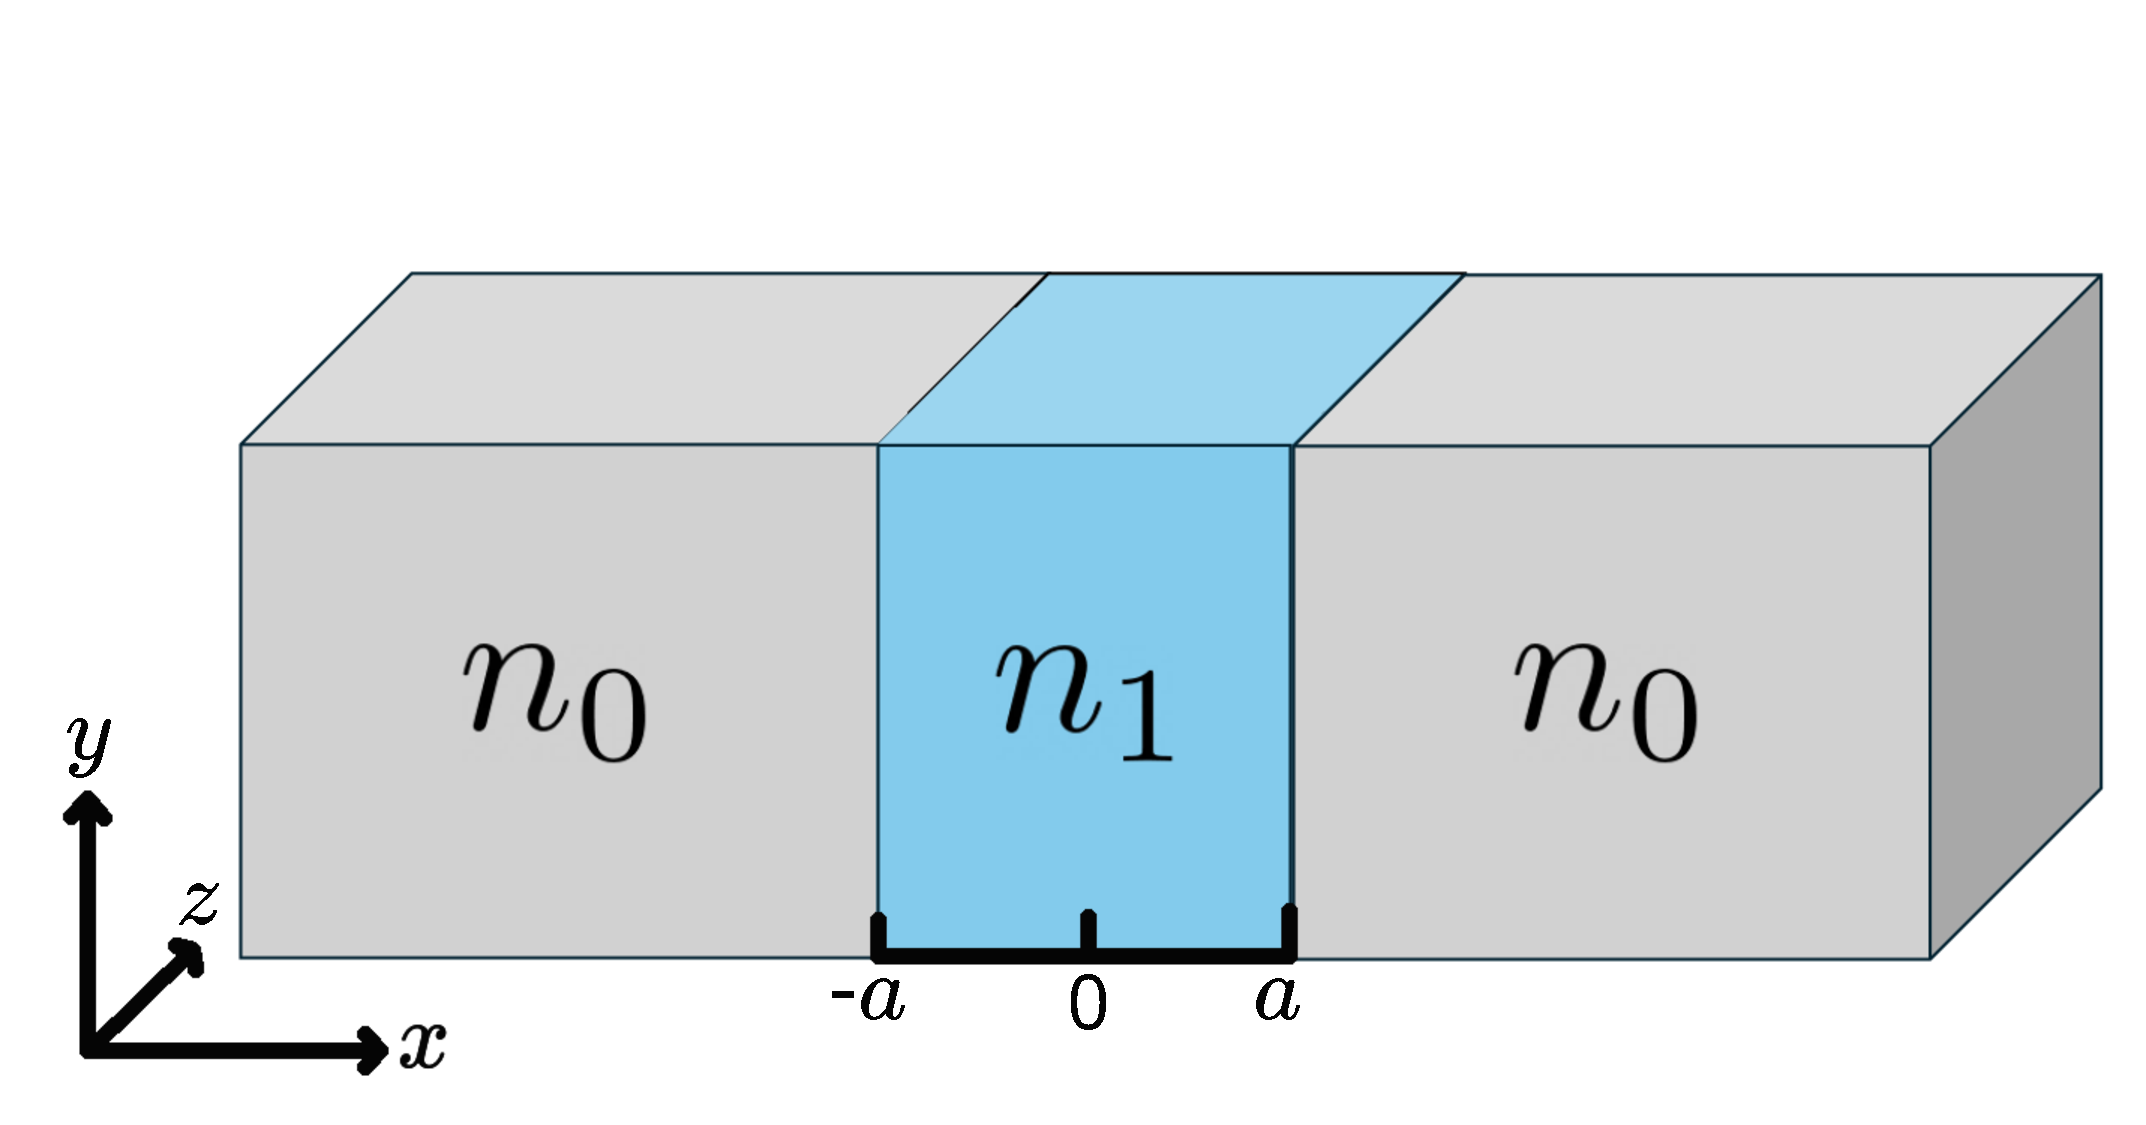
\includegraphics[width=0.6\linewidth]{media/slab.pdf}
	\caption[Forma de una guía de onda tipo losa.]{Forma de una guía de onda tipo losa. En las direcciones $\mathbf{\hat{y}}$ (vertical) y $\mathbf{\hat{z}}$ (hacia dentro de la página) la estructura es invariante.}
\end{figure}
\subsection{Modos TE}

Los modos transversales eléctricos o TE se pueden expresar como $\textbf{E}(x,z) =\mathbf{\hat{y}} E_y= \mathbf{\hat{y}} E(x)e^{i k_z z }$, donde se ha escogido polarización lineal en $\hat{\textbf{y}}$ para que el lado derecho de la ecuación (\ref{eqn:helmholz}) sea nulo y sea de tipo Helmholz:

\begin{align}
(\nabla^2  + k_0^2n^2) E(x)e^{ik_z z} &=  \left(\frac{\partial^2}{\partial x^2} + \frac{\partial^2}{\partial z^2} + k_0^2n^2\right) E(x)e^{ik_z z } 
\nonumber
\\
&= e^{ik_z z}\left[\frac{d^2  E(x)}{dx^2}  + (k_0^2n^2 -  k_z^2)E(x) \right]
\nonumber
\\
&=0
\nonumber
\\
\therefore \frac{d^2  E(x)}{dx^2}  + (k_0^2n^2 -  k_z^2)E(x) &= 0 \label{eqn:TEslab}
\end{align}

Para encontrar soluciones cuya energía esté localizada en la guía de onda y que decaiga fuera de ella, se impondrá $k_0^2n_0^2 < k_z^2 < k_0^2n_1^2$. Se hace natural definir $\alpha^2\equiv k_0^2n_1^2-k_z^2$ y $\beta^2\equiv k_z^2 - k_0^2n_0^2$. \textcolor{red}{Incluir cita Griffiths QM acerca de soluciones pares e impares para potencial real simétrico}. Si consideramos soluciones pares, la ecuación (\ref{eqn:TEslab}) tendrá soluciones

\begin{equation*}
	E(x) = \left\{\begin{matrix}
	E_{s1}\cos(\alpha x)\quad |x|\le a
	\\
	E_{s0}e^{-\beta|x|} \quad |x|>a
	\end{matrix}\right.
\end{equation*}

Por otro lado, las soluciones impares tienen la forma
\begin{equation*}
	E(x) = \left\{\begin{matrix}
	E_{a1}\sin(\alpha x)\quad |x|\le a
	\\
	E_{a0}e^{-\beta|x|} \quad |x|>a
	\end{matrix}\right.
\end{equation*}


Es necesario considerar las condiciones de interfase electromagnéticas. En este caso, continuidad de las componentes de \textbf{E} y \textbf{H} paralelas a la interfaz . A partir de la ecuación de Faraday-Lenz (\ref{eqn:faraday-lenz}) se tiene:

\begin{align*}
	\nabla\times\textbf{E} &= -\mu_0\frac{\partial \textbf{H}}{\partial t}
	\\
	\mathbf{\hat{z}}\partial_x E_y-\mathbf{\hat{x}}\partial_z E_y  &= i\omega \mu_0  \textbf{H}
	\\	
	\therefore \textbf{H}_{||} = -i\mathbf{\hat{z}}\frac{e^{ik_z z}}{\omega\mu_0}\frac{d E(x)}{dx}.
\end{align*}
Es decir, tanto $E(x)$ como $\frac{dE(x)}{dx}$ deben ser continuos en $|x|=a$. Aplicando esto en $x=a$ separadamente para las soluciones simétricas y antisimétricas:

\begin{align*}
E_{s1}\cos(\alpha a) &= E_{s0} e^{-\beta a} & E_{a1}\sin(\alpha a) &= E_{a0} e^{-\beta a}
\\
E_{s1}\alpha\sin(\alpha a) &= \beta E_{s0} e^{-\beta a} & E_{a1}\alpha\cos(\alpha a) &= -\beta E_{a0} e^{-\beta a}
\end{align*}

Al dividir las ecuaciones de abajo por las de arriba se elimina la dependencia en las amplitudes y se obtienen ecuaciones trascendentales para $k_z$:

\begin{align}
	\alpha a \tan(\alpha a) &= \beta a, & \alpha a \cot(\alpha a) &= -\beta a \label{eqn:trascendentalTE}
\end{align}

Usando las dos ecuaciones (\ref{eqn:trascendentalTE}) junto a la restricción $(\alpha a)^2 + (\beta a)^2 = k_0^2 a^2(n_1^2 - n_0^2) \equiv V^2$ es posible obtener soluciones gráficas para las constantes de propagación $k_z$.

\begin{figure}[H]
	\centering
	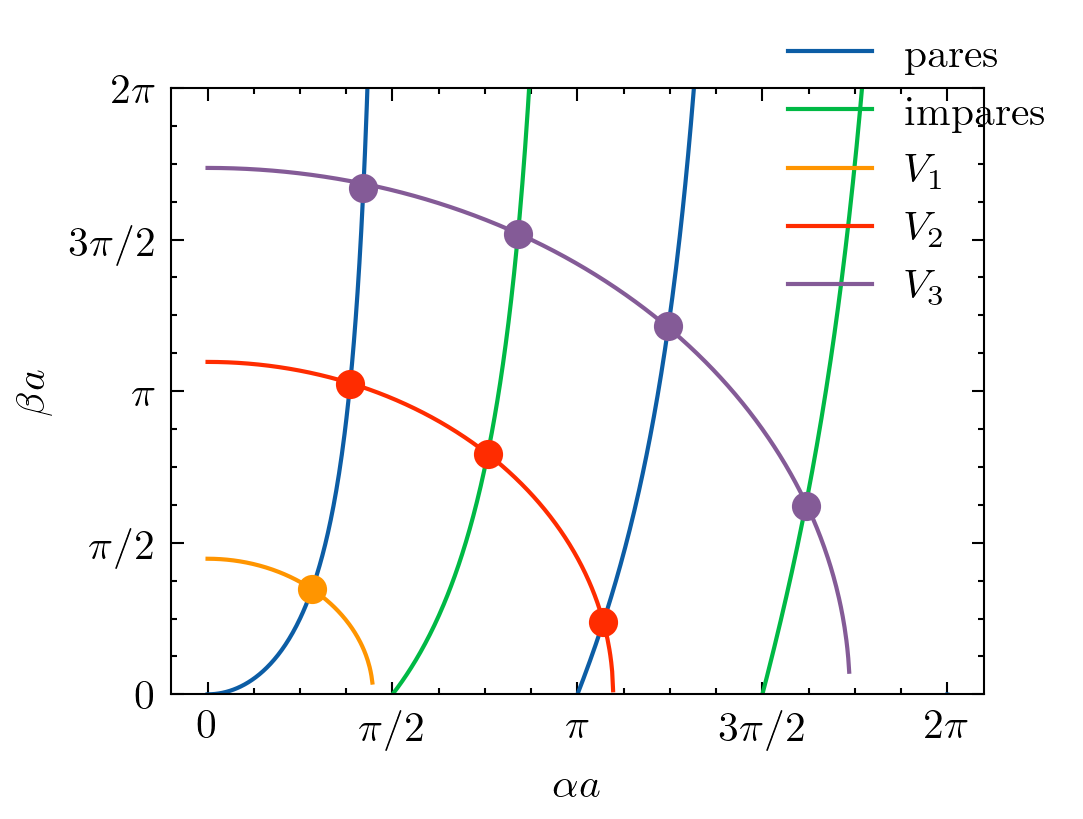
\includegraphics[width=0.7\linewidth]{media/slabgraphical}
	\caption[Soluciones gráficas de los modos TE]{Soluciones gráficas de los modos TE. A mayor contraste $\Delta n = n_1-n_0$, mayor cantidad de modos guiados soporta la guía de onda.}
\end{figure}
\subsection{Modos TM}
Los modos transversales magnéticos o TM se expresan como $\textbf{H}(x,z) =\mathbf{\hat{y}} H_y= \mathbf{\hat{y}} H(x)e^{i k_z z }$. Para expresar esta condición en términos del campo eléctrico $\textbf{E} = \textbf{E}_{||} + \textbf{E}_\perp$, se puede usar la ecuación de Ampère-Maxwell (\ref{eqn:ampere-maxwell}):

\begin{align*}
	\nabla\times\textbf{H} &= -\mathbf{\hat{x}} \partial_z H_y+ \mathbf{\hat{z}} \partial_x H_y = \mathbf{\hat{z}} e^{i k_z z }\frac{d H(x)}{dx} - \mathbf{\hat{x}} ik_z  e^{i k_z z } H(x)  
	\\	
	&= -i\omega\epsilon_0 n^2 \textbf{E}
	\\
	\therefore \textbf{E}_{||} = \mathbf{\hat{z}} \frac{ie^{i k_z z }}{n^2 \omega \epsilon_0} \frac{d H(x)}{dx}&,\quad \textbf{E}_\perp =  \mathbf{\hat{x}} \frac{k_z e^{i k_z z }}{n^2 \omega \epsilon_0 }   H(x).
\end{align*} 
Notemos que la ecuación (\ref{eqn:helmholz}) se puede separar por componentes, por lo que al considerar la ecuación que satisface la componente perpendicular $\textbf{E}_\perp$, se tiene:

\begin{align}
	(\nabla^2 + k_0^2 n^2) H_y
	&= \left(\frac{\partial^2}{\partial x^2} + \frac{\partial^2}{\partial z^2} + k_0^2n^2\right) H(x)e^{ik_z z }
	\nonumber
	\\
&= e^{ik_z z}\left[\frac{d^2  H(x)}{dx^2}  + (k_0^2n^2 -  k_z^2)H(x) \right]
\nonumber	
	\\	
	&= 0 
	\nonumber	
	\\
	\therefore 
	\frac{d^2  H(x)}{dx^2}  + (k_0^2n^2 -  k_z^2)H(x) &= 0
	\label{eqn:TMslab}
\end{align} 

La ecuación de modos TM (\ref{eqn:TMslab}) para $H(x)$ es idéntica que la ecuación (\ref{eqn:TEslab}) para $E(x)$ de modos TE. Es decir, definiendo $\alpha^2\equiv k_0^2n_1^2-k_z^2$ y $\beta^2\equiv k_z^2 - k_0^2n_0^2$ y considerando soluciones pares se tiene

\begin{equation*}
	H(x) = \left\{\begin{matrix}
	H_{s1}\cos(\alpha x)\quad |x|\le a
	\\
	H_{s0}e^{-\beta|x|} \quad |x|>a
	\end{matrix}\right.
\end{equation*}

Y las soluciones impares serán
\begin{equation*}
	H(x) = \left\{\begin{matrix}
	H_{a1}\sin(\alpha x)\quad |x|\le a
	\\
	H_{a0}e^{-\beta|x|} \quad |x|>a
	\end{matrix}\right.
\end{equation*}


Nuevamente, al considerar que $\textbf{H}_{||}= \mathbf{\hat{y}} H(x)e^{i k_z z }$ y $\textbf{E}_{||} = \mathbf{\hat{z}} \frac{ie^{i k_z z }}{n^2 \omega \epsilon_0} \frac{d H(x)}{dx}$ deben ser continuas, 

\begin{align*}
H_{s1}\cos(\alpha a) &= H_{s0} e^{-\beta a} & H_{a1}\sin(\alpha a) &= H_{a0} e^{-\beta a}
\\
H_{s1}\alpha\sin(\alpha a)/n_1^2 &= \beta H_{s0} e^{-\beta a}/n_0^2 & H_{a1}\alpha\cos(\alpha a)/n_1^2 &= -\beta H_{a0} e^{-\beta a}/n_0^2
\end{align*}

Al dividir las ecuaciones de abajo por las de arriba se elimina la dependencia en las amplitudes y se obtienen ecuaciones trascendentales implícitas en $k_z$:

\begin{align}
	\alpha a \tan(\alpha a)/n_1^2 &= \beta a/n_0^2, & \alpha a \cot(\alpha a)/n_1^2 &= -\beta a/n_0^2 \label{eqn:trascendentalTM}
\end{align}


\begin{figure}[H]
	\centering
	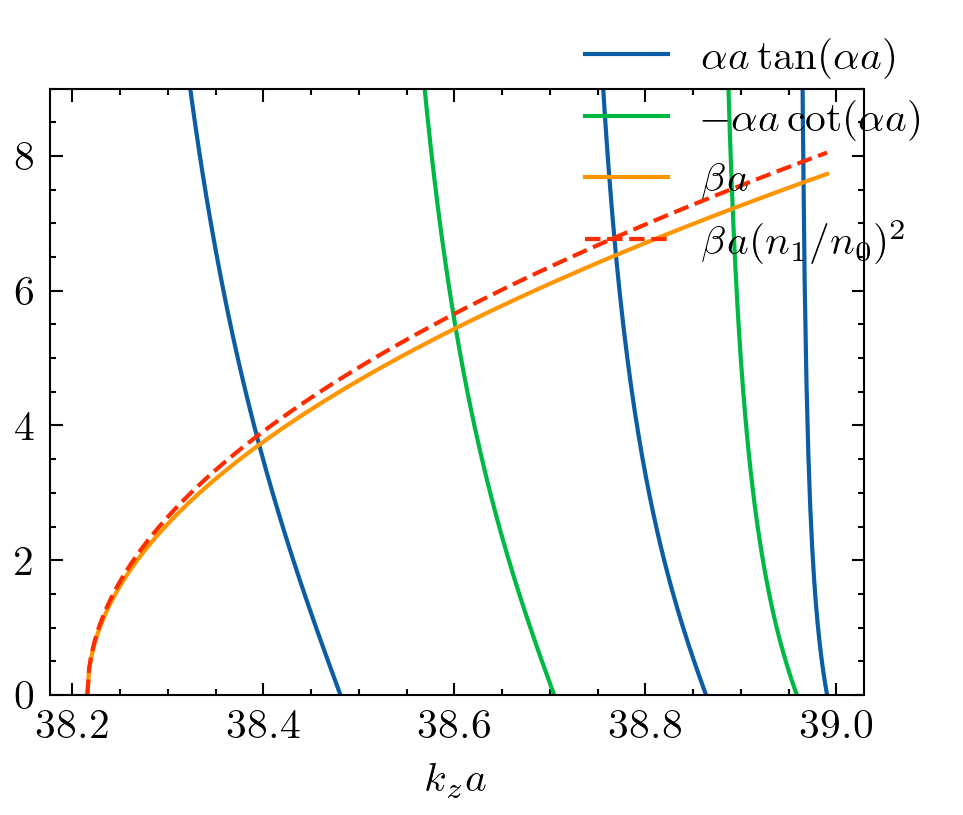
\includegraphics[width=0.7\linewidth]{media/slabgraphicalTETM1}
	\caption[Soluciones gráficas de los modos TE y TM]{Soluciones gráficas de los modos TE y TM para $\Delta n = 3\times 10^{-2}$. Se aprecia que las constantes de propagación de los modos TM (rojo discontinuo) son menores que las de los modos TE (naranjo liso).}
\end{figure}
\section{Soluciones analíticas para fibra óptica circular}
En la sección anterior se estudió el sistema más sencillo en el que se puede hablar de guías de onda dieléctricas. El siguiente paso en complejidad consiste en guías de onda circulares. Para ello, se considerará que el índice de refracción varía radialmente según 

\begin{equation}
	n( \rho ) = 
	\left\{\begin{matrix}
	n_1, \quad \text{si } \rho \le a
	\\
	n_0, \quad \text{si } \rho > a
	\end{matrix}\right.
	,\nonumber
\end{equation}
donde la tupla $(\rho, \phi, z)$ define las coordenadas cilíndricas a usar, más apropiadas para este problema. Al considerar las componentes longitudinales $\Psi$ = $E_z$,$H_z$ del campo eléctrico y magnético, respectivamente, usando separación de variables $\Psi =  R(\rho)\Phi(\phi) e^{ik_z z} $ la ecuación (\ref{eqn:helmholz}) toma la forma:

\begin{align}
	\left[\frac{\partial^2}{\partial \rho^2} + \frac{\partial}{\rho\partial \rho} + \frac{\partial^2}{\rho^2\partial \phi^2} +\left( k_0^2n^2 - k_z^2 \right)\right]  R(\rho)\Phi(\phi) = 0
	\nonumber
	\\
\rho^2\frac{d^2 R}{Rd\rho^2} + \rho\frac{dR}{Rd\rho} + \rho^2\left( k_0^2n^2 - k_z^2 \right) + \underbrace{\frac{d^2 \Phi}{\Phi d\phi^2}}_{-\ell^2} = 0
\nonumber
\\
\therefore \Phi(\phi) = A\cos(\ell\phi) + B\sin(\ell\phi)
\nonumber
\end{align}
Imponiendo condiciones de periodicidad $\Phi(0)=\Phi(2\pi)$ y $\Phi'(0)=\Phi'(2\pi)$, se tiene que $B=A\tan(\pi \ell)$, luego $0 = \tan(\ell \pi)$. Es decir, $\ell$ debe ser un número entero y $\Phi(\phi) = A\cos(\ell\phi)$.

La ecuación para $R(\rho)$ es de tipo Bessel, por lo que buscando soluciones tales que $k_0^2 n_0^2 < \beta_z^2 < k_0^2 n_1^2$ y definiendo nuevamente $\alpha^2 \equiv k_0^2n_1^2 - k_z^2$ y $\beta^2\equiv k_z^2 - k_0^2n_0^2$ se tiene:

\begin{align}
	\frac{d^2 R}{d\rho^2} + \frac{1}{\rho}\frac{dR}{d\rho} + \left( k_0^2n^2 - k_z^2 -\frac{\ell^2}{\rho^2}\right)R  = 0
	\nonumber
	\\
	\therefore R(\rho) = 
	\left\{
	\begin{matrix}	
	C_1 J_\ell (\alpha\rho) + D_1 Y_\ell (\alpha\rho), \quad \text{si } \rho \le a  
	\\
	C_2 K_\ell (\beta\rho) + D_2 I_\ell (\beta\rho), \quad \text{si } \rho > a  
	\end{matrix}
	\right.
	. \nonumber
\end{align}
Necesariamente se debe imponer $D_1 = D_2 = 0$ para que la solución sea finita para $\rho = 0$ y para $\rho \to +\infty$. Es decir, la parte radial de la solución es
\begin{align*}
 R(\rho) = 
	\left\{
	\begin{matrix}	
	C_1 J_\ell (\alpha\rho), \quad \text{si } \rho \le a  
	\\
	C_2 K_\ell (\beta\rho), \quad \text{si } \rho > a  
	\end{matrix}
	\right.
	. \nonumber
\end{align*}

En este caso, para imponer las condiciones de continuidad en $\textbf{E}_{||} = E_\phi \boldsymbol{\hat{\phi}} + E_z \hat{\textbf{z}}$ y $\textbf{H}_{||}= H_\phi \hat{\boldsymbol{\phi}} + H_z \hat{\textbf{z}}$, se hace necesario relacionar el resto de componentes del campo con $E_z$ y $H_z$. Explícitamente, las ecuaciones de Maxwell separando $\textbf{E}=\textbf{E}_\perp +\hat{\textbf{z}} E_z$ y $\textbf{H}=\textbf{H}_\perp +\hat{\textbf{z}} H_z$

\begin{align*}
	\left(\frac{1}{\rho}\frac{\partial E_z}{\partial \phi} - \frac{\partial E_\phi}{\partial z} \right)\hat{\boldsymbol{\rho}} + \left(\frac{\partial E_\rho}{\partial z} - \frac{\partial E_z}{\partial \rho} \right)\hat{\boldsymbol{\phi}} &= i\omega \mu_0\textbf{H}_\perp, & \frac{1}{\rho}\left(\frac{\partial (\rho E_\phi)}{\partial \rho} - \frac{\partial E_\rho}{\partial \phi} \right) &= i\omega \mu_0 H_z
	\\	
	\left(\frac{1}{\rho}\frac{\partial H_z}{\partial \phi} - \frac{\partial H_\phi}{\partial z} \right)\hat{\boldsymbol{\rho}} + \left(\frac{\partial H_\rho}{\partial z} - \frac{\partial H_z}{\partial \rho} \right)\hat{\boldsymbol{\phi}} &= -i\omega \epsilon_0 n^2 \textbf{E}_\perp, & \frac{1}{\rho}\left(\frac{\partial (\rho H_\phi)}{\partial \rho} - \frac{\partial H_\rho}{\partial \phi} \right) &= -i\omega \epsilon_0 n^2 E_z
	\\	
			\nabla_\perp \cdot \textbf{E}_\perp+  \textbf{E}_\perp \cdot \frac{\nabla_\perp n^2}{n^2}  &= -i k_z E_z, 
	&	
	\nabla_\perp\cdot\textbf{H}_\perp &= i k_z H_z,
\end{align*}


\section{Modos normales en guías de onda}

Si la estructura de guías de onda no varía en la dirección $z$, el campo eléctrico se puede expresar como una onda plana del tipo $\textbf{E}(\textbf{r}) = \textbf{E}_\nu(x, y) e^{i\beta_\nu z}$. A su vez, es conveniente separar el laplaciano como $\nabla^2 \equiv \nabla_\perp^2 + \frac{\partial^2}{\partial z^2}$. De esta forma, el lado izquierdo de las ecuaciones (\ref{eqn:helmholz}), se desarrolla como:

\begin{align}
	(\nabla^2  + k_0^2n^2) \textbf{E}(\textbf{r}) &= \left(\nabla_\perp^2 + \frac{\partial^2}{\partial z^2} + k_0^2n^2\right) \textbf{E}_\nu(x, y)  e^{i\beta_\nu z} \nonumber
\\	
	&= e^{i\beta_\nu z} \nabla_\perp^2 \textbf{E}_\nu -\beta_\nu^2\textbf{E}_\nu e^{i\beta_\nu z} + k_0^2n^2 \textbf{E}_\nu  e^{i\beta_\nu z}
\nonumber	
	\\	
	&= \left[  \nabla_\perp^2  + (k_0^2n^2-\beta_\nu^2) \right]\textbf{E}_\nu  e^{i\beta_\nu z}
	\nonumber	
	\\
	&\approx
	0
	\nonumber
	\\
	\therefore
	 \left[  \nabla_\perp^2  + k_0^2n^2(x,y) \right]&\textbf{E}_\nu(x,y)  = \beta_\nu^2 \textbf{E}_\nu(x,y), \label{eqn:eigenfield}
\end{align}
donde se ha usado la aproximación de guiaje débil para anular el lado de derecho de la ecuación (\ref{eqn:helmholz}). Notemos que la ecuación (\ref{eqn:eigenfield}) es un problema de autovalores $\beta_\nu^2$ y autofunciones $\textbf{E}_\nu(x,y)$, que son ortogonales y forman una base completa (ver apéndice \ref{sec:orto}). En principio, la forma espacial del índice de refracción $n(x, y)$ puede ser arbitraria siempre y cuando que se satisfaga la condición de guiaje débil. 

\section{Teoría de modos acoplados}
	Para el estudio de redes fotónicas, es conveniente utilizar herramientas similares a las de la Física del Sólido en lo que respecta a potenciales periódicos. En particular, se puede suponer que los modos guiados de una guía de onda están fuertemente ligados a ella (enlace fuerte o \textit{Tight Binding}), incluso en presencia de otras guías de onda. Es decir, se supondrá que el $\nu$-ésimo modo de la $m$-ésima guía de onda satisface para toda distancia de propagación $z$ la ecuación (\ref{eqn:eigenfield}), donde el índice de refracción total se puede descomponer en una suma periódica de guías de onda $n^2(\textbf{r}) = \sum_{m} n^2_m(\textbf{r})$. Entonces, descomponiendo el campo eléctrico total de la forma $\textbf{E}(\textbf{r}) = \sum_{\nu, m} \textbf{E}_{\nu, m}(x, y) a_{\nu, m}(z) e^{i\beta_{\nu, m} z}$ y reemplazando en la ecuación (\ref{eqn:helmholz}) se tiene:

\begin{align}
	(\nabla^2  + k_0^2n^2) \textbf{E}(\textbf{r}) &= \left(\nabla_\perp^2 + \frac{\partial^2}{\partial z^2} + k_0^2n^2 \right)\sum_{\nu, m} \textbf{E}_{\nu, m}(x, y) a_{\nu, m}(z) e^{i\beta_{\nu, m} z}
	\nonumber
	\\
	&= \sum_{\nu, m} \left[a_{\nu, m} e^{i\beta_{\nu, m} z} \left(\nabla_\perp^2 +k_0^2n^2 \right)\textbf{E}_{\nu, m} + \textbf{E}_{\nu, m}\frac{d^2}{d z^2}\left(a_{\nu, m} e^{i\beta_{\nu, m} z}\right)\right]
	\nonumber	
	\\
	&= \sum_{\nu, m} \left[a_{\nu, m}  \left(\nabla_\perp^2 +k_0^2n^2 -\beta_{\nu,m}^2 \right) + \frac{d^2 a_{\nu, m}}{d z^2}  +2i\beta_{\nu,m}\frac{d a_{\nu, m}}{d z} \right]e^{i\beta_{\nu, m} z}\textbf{E}_{\nu, m}
		\nonumber	
	\\
	&\approx \sum_{\nu, m} \left[a_{\nu, m}  k_0^2(n^2 - n^2_{m}) +2i\beta_{\nu,m}\frac{d a_{\nu, m}}{d z} \right]e^{i\beta_{\nu, m} z}\textbf{E}_{\nu, m}
	\nonumber	
	\\
	&= 0,
	\nonumber	
\end{align}
Donde se ha usado que $\left|\frac{d^2 a_{\nu, m}}{d z^2}\right|\ll 2\beta_{\nu,m}\left|\frac{d a_{\nu, m}}{d z}\right|  $, conocida como aproximación paraxial. Aplicando producto punto con $\textbf{E}_{\mu, m'}^*$ e integrando en todo el plano $xy$:
\begin{align}
	  \int\displaylimits_{-\infty}^{+\infty}\int\displaylimits_{-\infty}^{+\infty} \sum_{\nu, m} \left[a_{\nu, m}  k_0^2(n^2 - n^2_{m}) +2i\beta_{\nu,m}\frac{d a_{\nu, m}}{d z} \right]e^{i\beta_{\nu, m} z}\textbf{E}_{\nu, m} \cdot \textbf{E}_{\mu, m'}^* dxdy &= 0
	  \nonumber
	  \\
	  \sum_{\nu, m} \left(2i\beta_{\nu,m}\frac{d a_{\nu, m}}{d z} \delta_{\nu,\mu}\delta_{m,m'} +  2\beta_{\mu, m'}C_{m', m, \nu, \mu}   a_{\nu, m} \right)e^{i\beta_{\nu, m} z} &= 0
	  \nonumber
	  \\
	  	  i\frac{d a_{\mu, m'}}{d z} e^{i\beta_{\mu, m'} z} +  \sum_{\nu, m\neq m'}C_{m', m, \nu, \mu}   a_{\nu, m} e^{i\beta_{\nu, m} z} &= 0
	\label{eqn:CMT1}
\end{align}
donde se han definido y usado
\begin{align*}
	   C_{m', m, \nu, \mu} &\equiv \frac{k_0^2}{2\beta_{\mu, m'}}\int\displaylimits_{-\infty}^{+\infty}\int\displaylimits_{-\infty}^{+\infty} (n^2 - n^2_{m}) \textbf{E}_{\nu, m} \cdot \textbf{E}_{\mu, m'}^* dxdy , \quad\int\displaylimits_{-\infty}^{+\infty}\int\displaylimits_{-\infty}^{+\infty} \textbf{E}_{\nu, m} \cdot \textbf{E}_{\mu, m'}^* dxdy \approx \delta_{\nu,\mu}\delta_{m,m'}.
\end{align*}
Es decir, el efecto del modo $(\nu, m)$ en la dinámica del modo $(\mu, m')$ sólo es apreciable al ponderar con la expresión $(n^2 - n^2_{m})$, lo que da origen al término $C_{m', m, \nu, \mu}$ conocido comúnmente como constante de acoplamiento. Sin el peso del contraste, la interacción es evanescente, por lo que la aproximación de ortogonalidad se hace razonable con suficiente distancia entre guías (sobre los 15 $\mu$m en los experimentos de esta tesis). Cuando $m=m'$, el acoplamiento $C_{m', m, \nu, \mu}$ es nulo por definición. Es por ello que no se incluye en la sumatoria de la ecuación (\ref{eqn:CMT1}). 

Para fijar ideas, consideremos el caso del dímero monomodal homogéneo, considerando una distancia $d$ entre guías \textcolor{red}{INCLUIR ESQUEMA PARA EXPLICAR ACOPLAMIENTO}. El índice de refracción en este caso es $n^2 = n_1^2 + n_2^2$, con $n_1^2(\textbf{r})=n_2^2(\textbf{r}+\textbf{d})$. Dada la simetría del problema, la constante de acoplamiento se puede desarrollar como 
\begin{align}
	C_{1, 2} &=  \frac{1}{2\beta}\int\displaylimits_{-\infty}^{+\infty}\int\displaylimits_{-\infty}^{+\infty} k_0^2 n_1^2(\textbf{r}) \textbf{E}_{2}(\textbf{r}) \cdot \textbf{E}_{1}^*(\textbf{r}) dxdy 
	= \frac{k_0^2}{2\beta}\int\displaylimits_{-\infty}^{+\infty}\int\displaylimits_{-\infty}^{+\infty}  n_2^2(\textbf{r}+\textbf{d}) \textbf{E}_{1}(\textbf{r}+\textbf{d}) \cdot \textbf{E}_{1}^*(\textbf{r}) dxdy 
	\nonumber	
	\\	
	&= \frac{k_0^2}{2\beta}\int\displaylimits_{-\infty}^{+\infty}\int\displaylimits_{-\infty}^{+\infty} n_2^2(\textbf{r}) \textbf{E}_{1}(\textbf{r}) \cdot \textbf{E}_{1}^*(\textbf{r}-\textbf{d}) dxdy 
	= \frac{k_0^2}{2\beta}\int\displaylimits_{-\infty}^{+\infty}\int\displaylimits_{-\infty}^{+\infty} n_2^2(\textbf{r}) \textbf{E}_{1}(\textbf{r}) \cdot \textbf{E}_{2}^*(\textbf{r}) dxdy 
	\nonumber
	\\	
	&= C_{2,1} \equiv C
	\nonumber
\end{align}
 por lo que las dos ecuaciones dinámicas se escriben como:

\begin{equation}
	i\frac{d a_1}{dz} + C a_2 = 0, \quad\quad i\frac{d a_2}{dz} + C a_1 = 0 \nonumber
\end{equation}


	

\chapter{Métodos numéricos}
\section{COMSOL (elementos finitos)}
A partir de la ecuación (\ref{eqn:rotordoble}) y separando el campo eléctrico $\textbf{E}(\textbf{r}) = \textbf{E}_1(\textbf{r}) e^{-i \phi_1 (\textbf{r})}$ en una envolvente lenta $\textbf{E}_1(\textbf{r})$ y una fase rápidamente oscilante $\phi_1 (\textbf{r})$ ,

\begin{align}
\nabla\times[\nabla\times(\textbf{E}_1 e^{-i \phi_1 })] &=  n^2k_0^2 \textbf{E}_1 e^{-i \phi_1}
\\
\nabla\times[ e^{-i \phi_1} \times (\nabla \times \textbf{E}_1) + \nabla(e^{-i \phi_1})\times \textbf{E}_1] &=  n^2k_0^2 \textbf{E}_1 e^{-i \phi_1}
\\
\nabla\times[ e^{-i \phi_1}  (\nabla  - i  \textbf{k} _1)\times\textbf{E}_1  ] &=  n^2k_0^2 \textbf{E}_1 e^{-i \phi_1}
\\
e^{-i \phi_1}  \nabla\times[ (\nabla  - i  \textbf{k} _1)\times\textbf{E}_1] + \nabla(e^{-i \phi_1})\times  (\nabla  - i  \textbf{k} _1)\times\textbf{E}_1  &=  n^2k_0^2 \textbf{E}_1 e^{-i \phi_1}
\\
e^{-i \phi_1}  \nabla\times[ (\nabla  - i  \textbf{k} _1)\times\textbf{E}_1] - i\textbf{k}_1 e^{-i \phi_1}\times  (\nabla  - i  \textbf{k} _1)\times\textbf{E}_1  &=  n^2k_0^2 \textbf{E}_1 e^{-i \phi_1}
\\
	(\nabla-i\textbf{k}_1)\times((\nabla-i\textbf{k}_1)\times \textbf{E}_1) &= n^2k_0^2 \textbf{E}_1,
	 \label{eqn:comsol}
\end{align}
con $\textbf{k}_1 = \nabla\phi_1(\textbf{r})$.
La ecuación (\ref{eqn:comsol}) se puede resolver vía el software comercial COMSOL \textit{Multiphysics} mediante elementos finitos más gruesos que los que se tendría que usar a partir de la ecuación (\ref{eqn:rotordoble}) debido a la separación entre envolvente y fase, sin haber hecho aproximación alguna.

\section{Expansión en modos normales}

\section{Beam Propagation Method} 

Por otro lado, utilizando la aproximación paraxial escogiendo el eje $z$  como dirección de propagación y seleccionando la polarización horizontal del campo, es posible simplificar la ecuación (\ref{eqn:comsol}) y llegar a la formulación de un método numérico escalar conocido como \textit{Beam Propagation Method}, utilizado ampliamente en esta área de investigación \cite{bics, interorbital, OAMCaging, vortex, bpm}. Éste consiste en resolver numéricamente la ecuación
\begin{equation}
	2in_0k_0\frac{\partial}{\partial z}\psi(x,y,z) = \nabla_\perp^2 \psi (x,y,z) + \left(n^2-n_0^2\right)k_0^2 \psi (x,y,z), \label{eqn:paraxial}
\end{equation}
con $\psi(x,y,z)$, $n_0$ , $n(x,y)$ y $k_0$ la envolvente de la componente horizontal campo eléctrico, el índice de refracción del material, el índice de refracción inducido y el número de onda en el vacío, respectivamente. 

\section{Teoría de modos acoplados}

Aplicando teoría acoplada de modos \cite{coupledmodetheory} a la ecuación (\ref{eqn:paraxial}), con el objetivo de describir de forma discreta una red fotónica, es posible derivar las llamadas ecuaciones discretas tipo Schrödinger \cite{discretesolitons, artificialFB, FBdynamics}
\begin{equation}
	-i\frac{\partial u_{\vec{n}} }{\partial z} = \beta_{\vec{n}}u_{\vec{n}} + \sum_{\vec{m}\neq\vec{n}} C_{\vec{n},\vec{m}}u_{\vec{m}}, \label{eqn:CMT}
\end{equation}
con $u_{\vec{n}}, \beta_{\vec{n}}$ y $C_{\vec{n}, \vec{m}}$ la envolvente normalizada del campo eléctrico, la constante de propagación normalizada y las constantes de acoplamiento entre los modos de las guías en las posiciones de la red $\vec{n}$ y $\vec{m}$, respectivamente.

\chapter{Métodos Experimentales}

En este capítulo se detallan los procedimientos experimentales desarrollados para la fabricación y caracterización de redes fotónicas basadas en guías de onda. La metodología comprende tres aspectos fundamentales: (1) escritura directa de guías mediante láser femtosegundo, (2) sistemas de excitación óptica con láser supercontinuo, y (3) técnicas avanzadas de modulación espacial de luz para el control de condiciones iniciales.


\section{Escritura directa de guías de onda \label{cap:fs}}

La fabricación de guías de onda se realizó mediante la técnica de escritura directa con láser femtosegundo. Este método permite crear estructuras tridimensionales en sustratos de vidrio mediante el efecto de cambio de índice de refracción inducido por láser \citep{femto_writing}.

\begin{figure}[H]
    \centering
    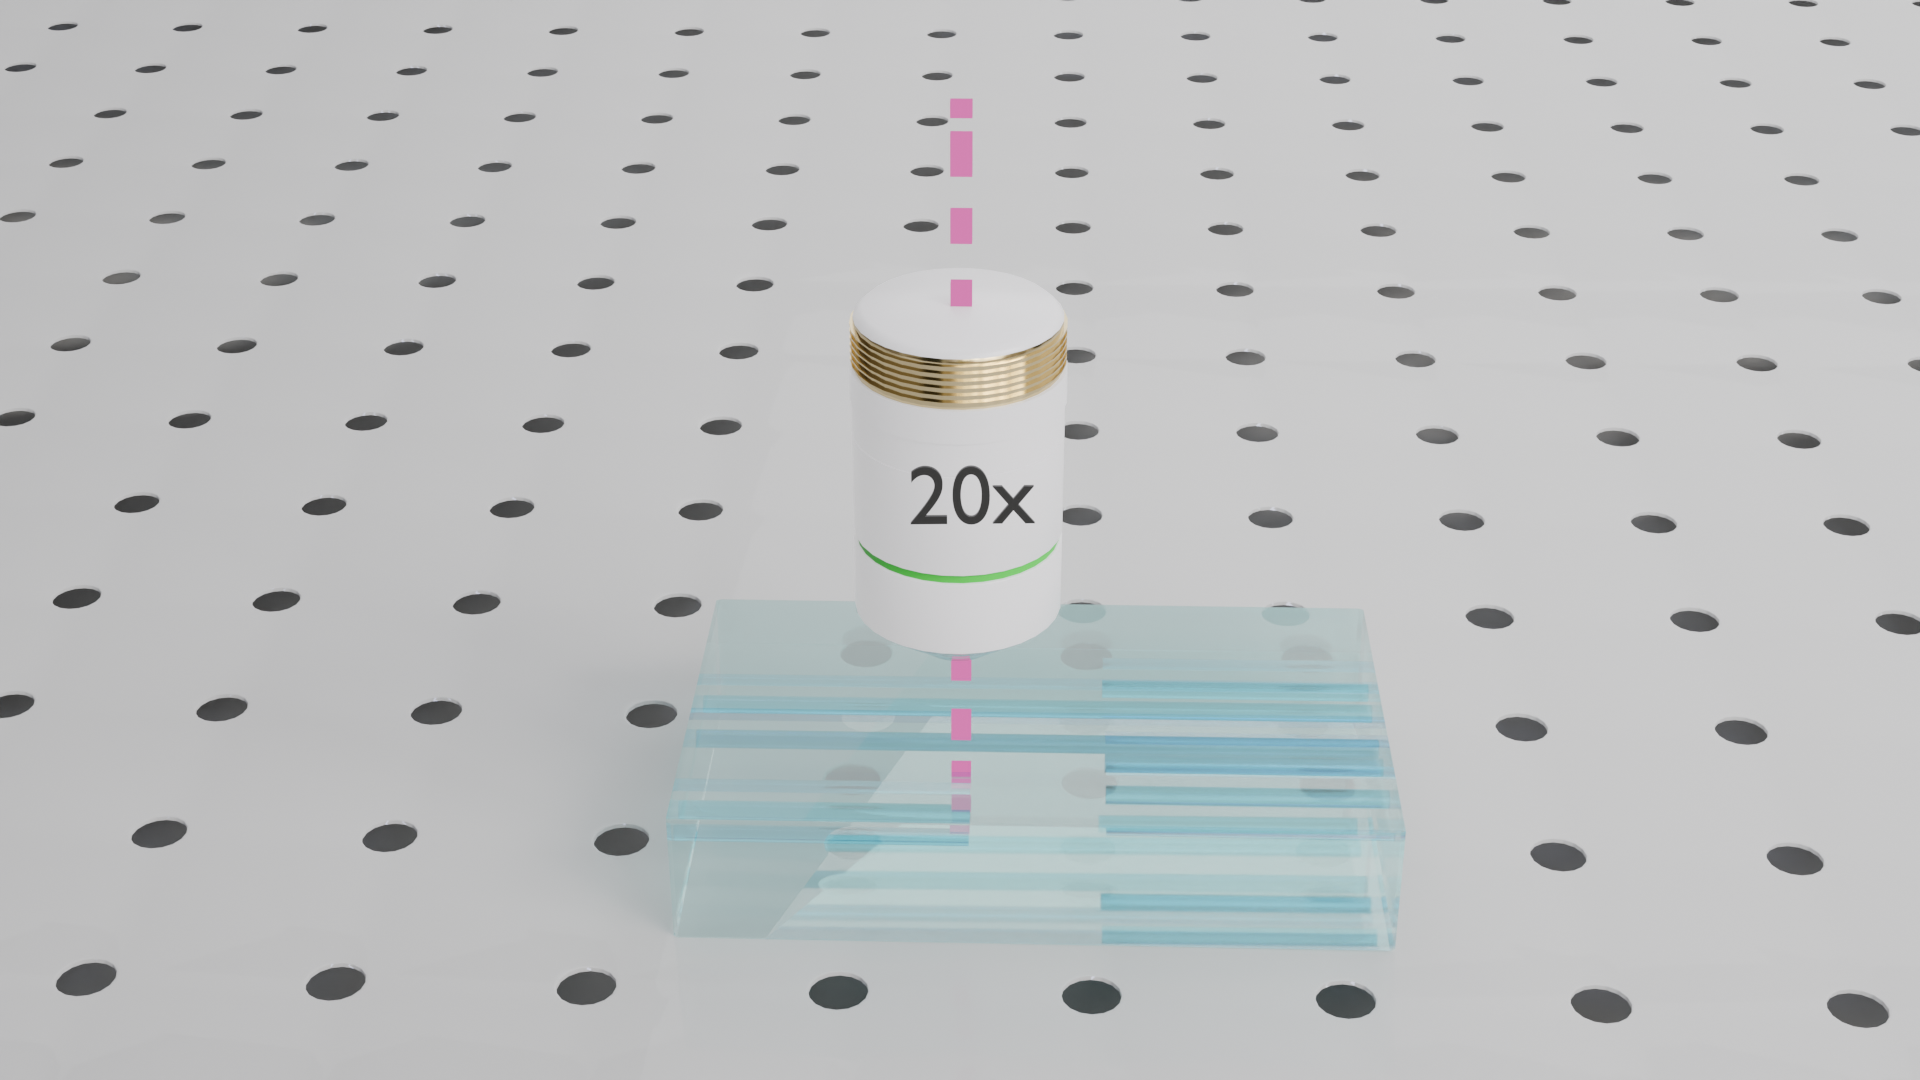
\includegraphics[width=0.6\linewidth, trim={18cm 4cm 15cm 6cm},clip]{media/fabrication1}
    \caption[Esquema de la técnica de escritura de guías de onda.]{Esquema de la técnica de escritura de guías de onda. El haz láser es focalizado mediante objetivo microscópico (20x) mientras la muestra se desplaza en tres ejes mediante una plataforma controlada por computadora.}
\end{figure}

Los parámetros de escritura que funcionan para excitar modos en el espectro visible son:
\begin{itemize}
    \item Tasa de repetición: 1 kHz.
    \item Velocidad de escritura: 0.1 - 10 mm/s.
    \item Potencia de llegada medida: 10.0 - 16.0 mW (90.0 - 144.0 mW).
\end{itemize}

\section{Montaje de excitación láser supercontinuo}

Para la caracterización óptica se implementó un sistema de excitación basado en un láser supercontinuo (SC) de banda ancha (450-2400 nm). Específicamente, el modelo es un YSL SC-5. La configuración permite seleccionar longitudes de onda específicas mediante un modulador acústico AOTF-PRO, con una resolución espectral de $\pm$5 nm y una potencia de salida de 1 mW por longitud de onda.

\begin{figure}[H]
    \centering
    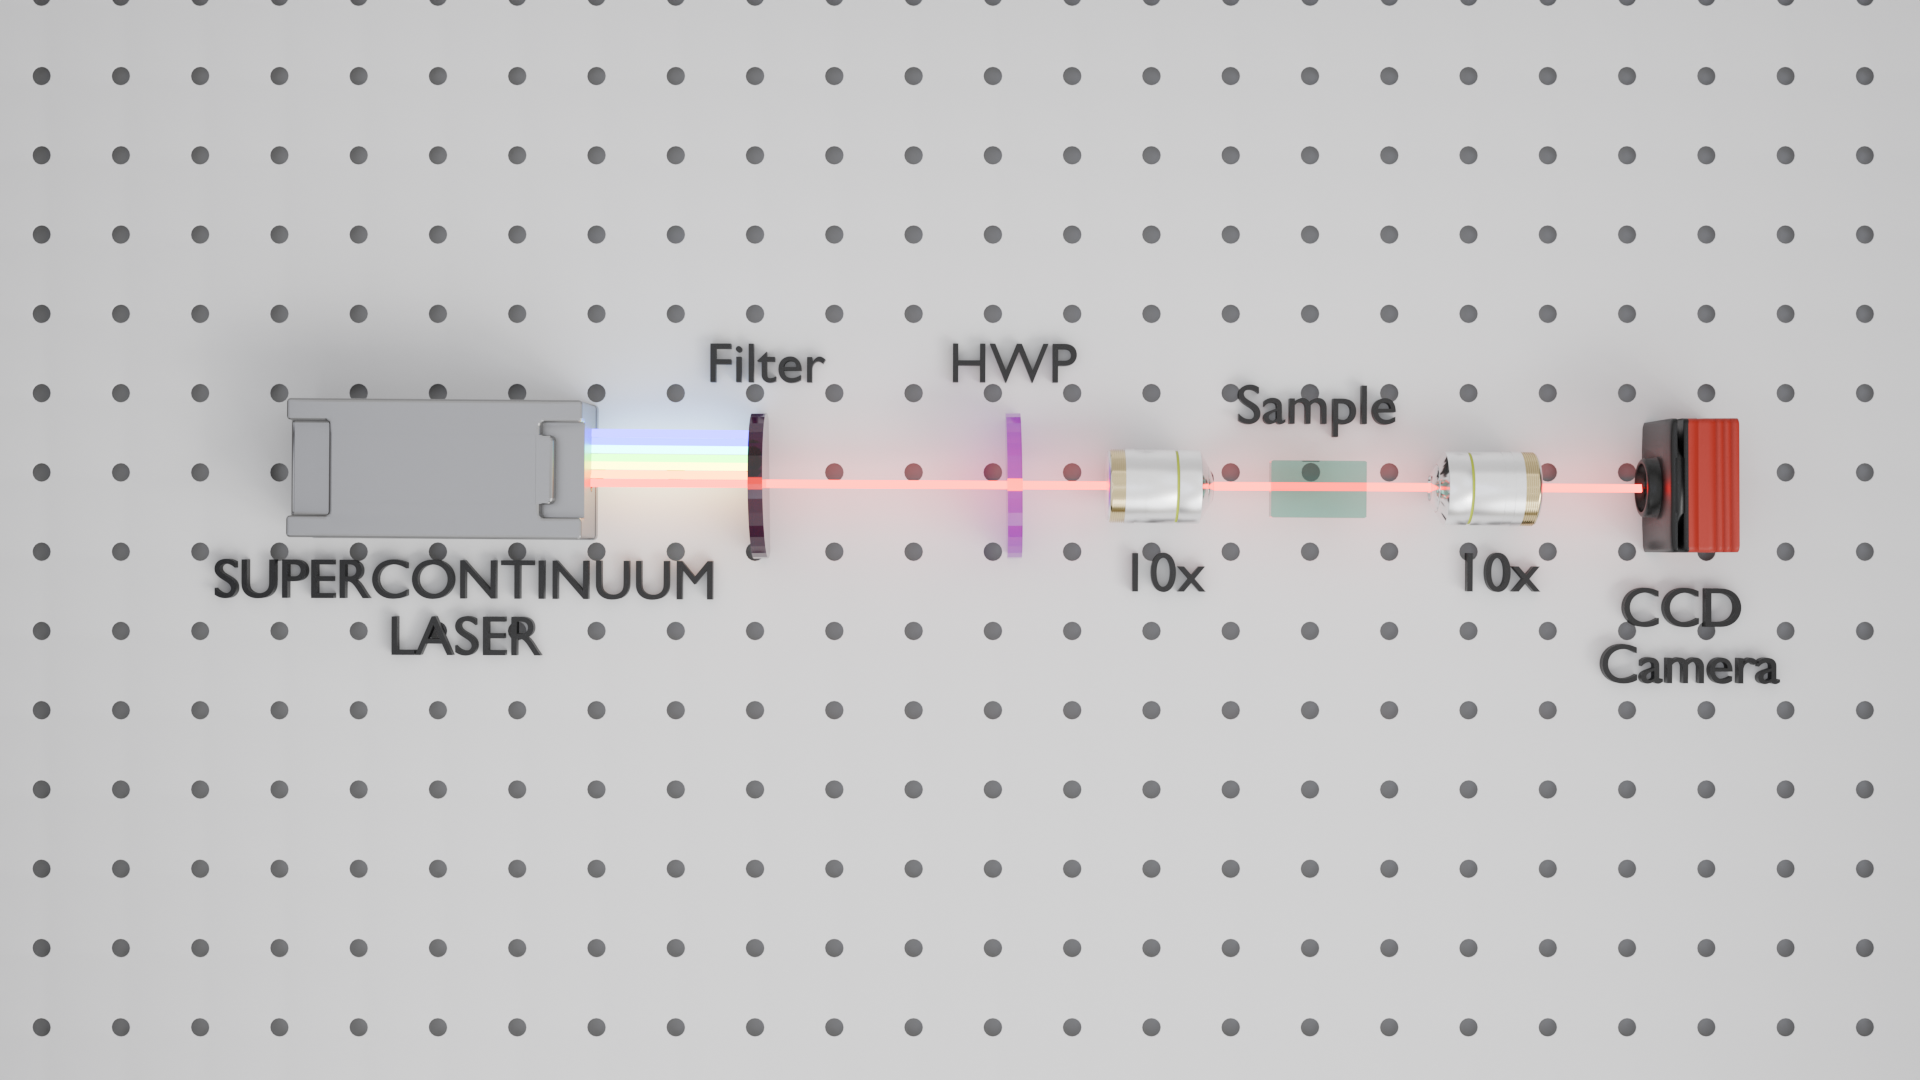
\includegraphics[width=\linewidth, trim={5cm 9cm 3cm 7cm},clip]{media/SC_setup}
    \caption{Montaje de excitación por láser supercontinuo.}
\end{figure}

\section{Montaje de modulación espacial de luz}

Para usar condiciones iniciales distintas a una gaussiana se hace necesario incorporar métodos de modulación espacial de luz. En esta tesis se utilizó una técnica conocida como grabado de fase mediante holograma \citep{terhalle}.

\subsection{Etapa premodulación}
El modulador espacial de luz utilizado es un HOLOEYE PLUTO-NIR SLM - Reflective LCOS (resolución 1920$\times$1080 px, tamaño de píxel 8 $\mu$m), cuya respuesta óptica ocurre con polarización paralela al plano de la mesa óptica. Se utiliza un retardador de media onda ($\lambda/2$) seguido de un polarizador Glan-Thompson 100.000:1 con el objetivo de que la polarización de la luz láser coincida con la de la respuesta del SLM. Posteriormente se magnifica y se colima el haz para que abarque todo el área de pixeles disponible con un par de lentes 20x y $L_1$ de foco 100mm (telescopio).

\subsection{Etapa de modulación}
Una rejilla de difracción que maximiza la potencia del primer orden de difracción es utilizada. Para modular en amplitud se debe multiplicar la rejilla por la máscara de amplitud deseada, mientras que para modular en fase basta con sumar el nivel de gris correspondiente a la fase deseada. En la Figura \ref{fig:SLMblaze} se bosqueja el algoritmo implementado en Python en el anexo \ref{sec:codigoSLM}.

{
\sidecaptionvpos{figure}{c}
\begin{SCfigure}[]
    \centering
    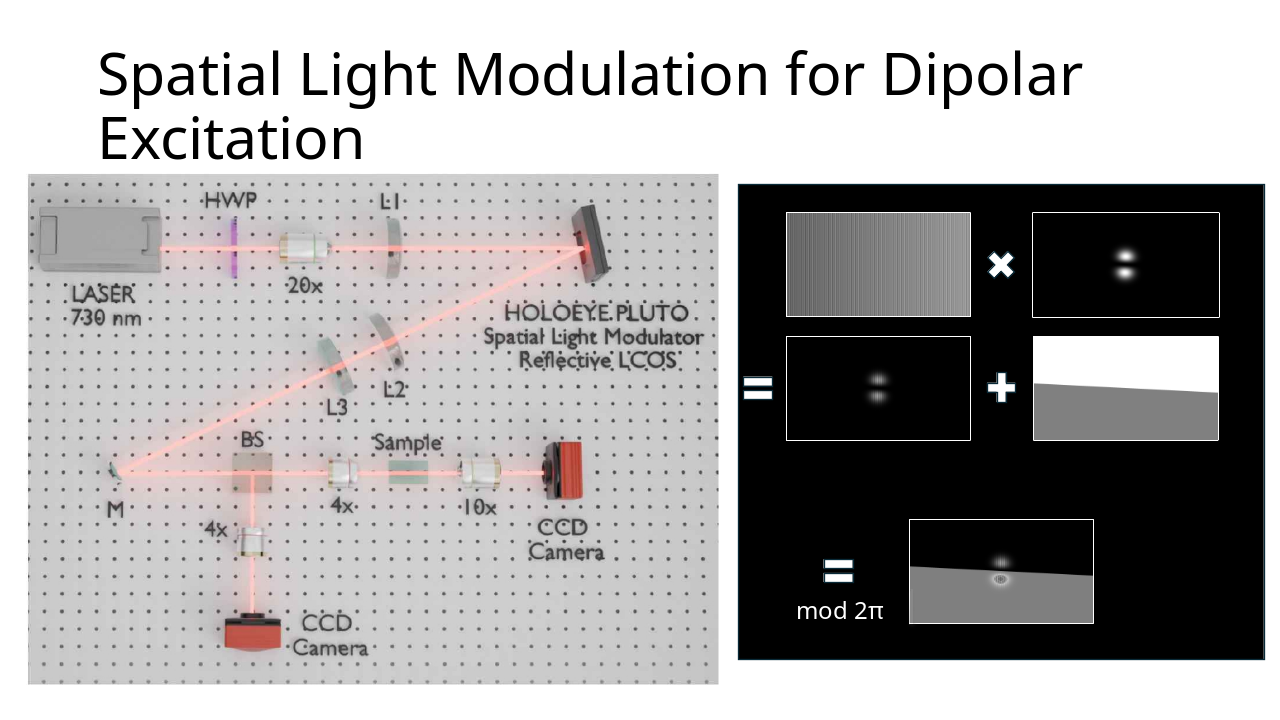
\includegraphics[width=0.4\linewidth, trim={19.5cm 0 0 5cm}, clip]{media/SLMblaze4.png}
    \caption[Modulación espacial de luz para máscaras de amplitud y fase arbitrarias.]{Algoritmo de modulación espacial de luz para máscaras de amplitud y fase arbitrarias. Los parámetros de la rejilla de difracción están sujetos a la longitud de onda usada (730 nm).\label{fig:SLMblaze}}
\end{SCfigure}
}

\subsection{Etapa de acoplamiento}
La imagen modulada pasa por un par de lentes $L_2$ de foco 1000 mm y $L_3$ de foco 50 mm para reducir el tamaño al orden de los micrómetros. La inclinación de la cara de entrada de la muestra debe coincidir con el plano de la imagen modulada, por lo que se generan dos pares de haces gaussianos, unos verticales y otros horizontales, de manera de que al trasladar el lente objetivo 4x, los máximos de difracción se generen en el centro de los haces gaussianos.

\subsection{Etapa de captura en cámara}
Una vez calibrada la inclinación de la muestra, se fija su posición. Un lente objetivo 10x permite magnificar la imagen de salida y capturar los resultados en un Beam Profiler modelo BC106N-VIS con resolución espacial de 6.45 $\mu$m/píxel \citep{thorlabs_beam_profiler}.

Opcionalmente, se puede intervenir el montaje para superponer un interferómetro tipo Mach-Zehnder. Para ello, se debe colocar un Beam Splitter entre el lente $L_1$ y el SLM para usar el haz previo a la modulación como referencia. Para recombinar los haces y hacerlos interferir, se debe colocar otro Beam Splitter entre el obejtivo 10x y la cámara final. Dado que el haz de referencia tiende a ser más potente que la luz propagada, suele requerirse además un filtro de densidad neutra (ND-Filter) para equiparar ambos haces.

\subsection{Circuito óptico}
\begin{figure}[H]
    \centering
    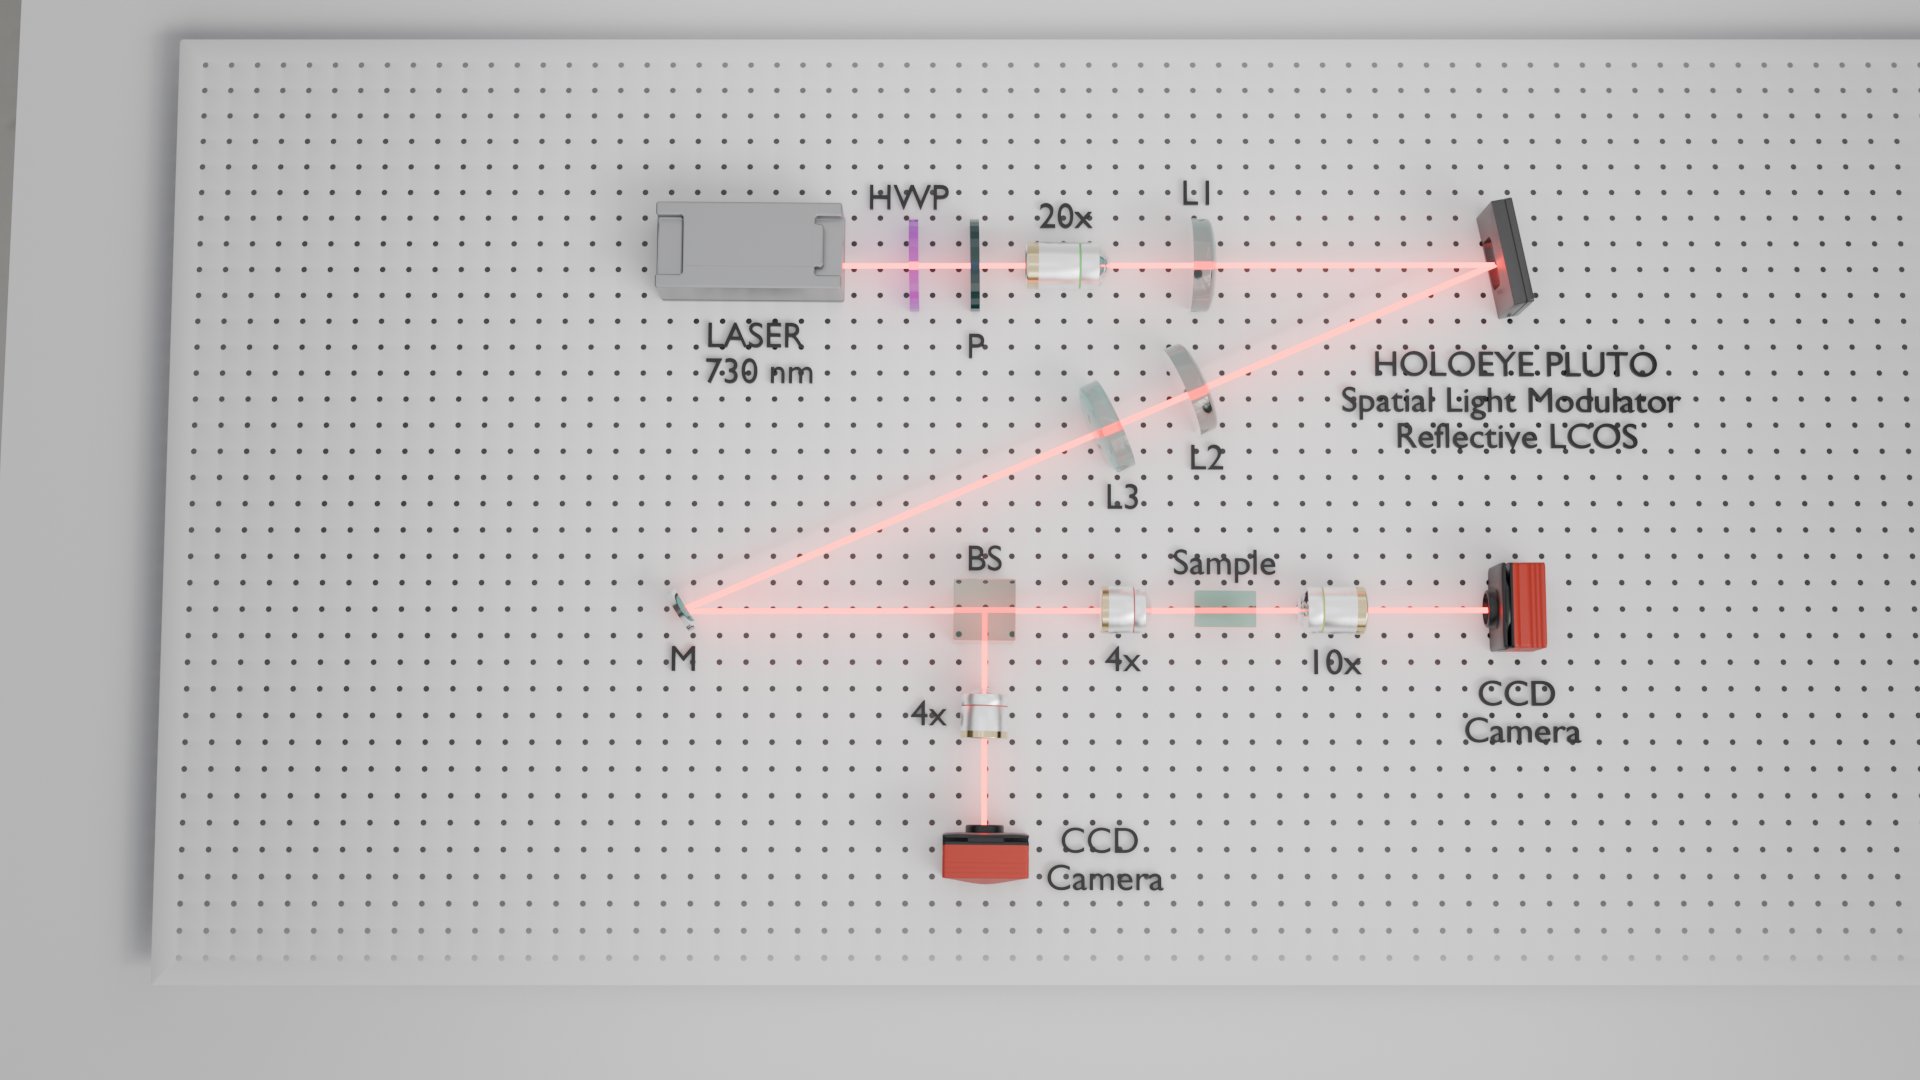
\includegraphics[width=\linewidth, trim={21cm 5cm 7cm 5cm},clip]{media/SLM_setupv1}
    \caption{Diagrama completo del sistema de modulación espacial.}
\end{figure}

\section{Análisis de imágenes \label{sec:analimag}}
A partir de las imágenes capturadas es posible extraer información de la potencia que contiene cada sitio del sistema fotónico discreto en estudio. Para ello la imagen completa debe ser seccionada equispaciadamente en rectángulos que encierren las regiones donde existen guías de onda, iluminadas o no. La potencia de cada sitio será entonces la suma de la intensidad de cada píxel encerrado en su rectángulo respectivo.

El procesamiento de imágenes incluye:
\begin{itemize}
    \item Corrección de fondo
    \item Normalización por intensidad máxima.
    \item Segmentación automática mediante umbral.
\end{itemize}

Los datos obtenidos permiten reconstruir la distribución de potencia en la red fotónica y analizar fenómenos de acoplamiento entre guías vecinas.
\chapter{Acoplamiento de modos $p_y$ y ángulo de invisibilidad \label{cap:invisibility}}

En electrostática, es posible describir las interacciones dipolares eléctricas mediante los polinomios de Legendre de orden 2, $P_2(\cos\theta) = 3\cos^2\theta - 1$, donde $\theta$ representa el ángulo entre los dipolos. El valor $\theta_m \approx 0.62$ radianes se denomina \textit{ángulo mágico}, ya que anula el término de interacción dipolar \citep{medmagic}.

Este capítulo se centra en los modos dipolares verticales o también llamados modos $p_y$, cuya excitación requiere superar la condición de corte (longitud de onda suficientemente pequeña junto con un contraste $\Delta n$ y un ancho de guía suficientemente grandes).
\section{Acopladores}
Al estudiar el acoplamiento entre modos $p_y$ en guías elípticas, se distinguen dos casos límite: para acopladores horizontales, el acoplamiento $\varkappa_\pi$ presenta signo positivo, mientras que para acopladores verticales, el acoplamiento $\varkappa_\sigma$ tiene signo negativo \cite{Pmodecoupling}.
Este comportamiento es análogo al observado en los enlaces químicos $\sigma$ y $\pi$ de las cadenas de carbono orgánicas. Para verificar este efecto, se fabricaron 20 dímeros con una separación de 25 $\mu$m y una distancia de propagación de 15 mm, variando el ángulo entre guías desde 0.00 rad hasta 1.57 rad. Mediante un modulador espacial de luz (SLM), se generó un modo P caracterizado por dos lóbulos de igual tamaño con una diferencia de fase de $\pi$ entre ellos.
\begin{figure}[H]
    \centering
    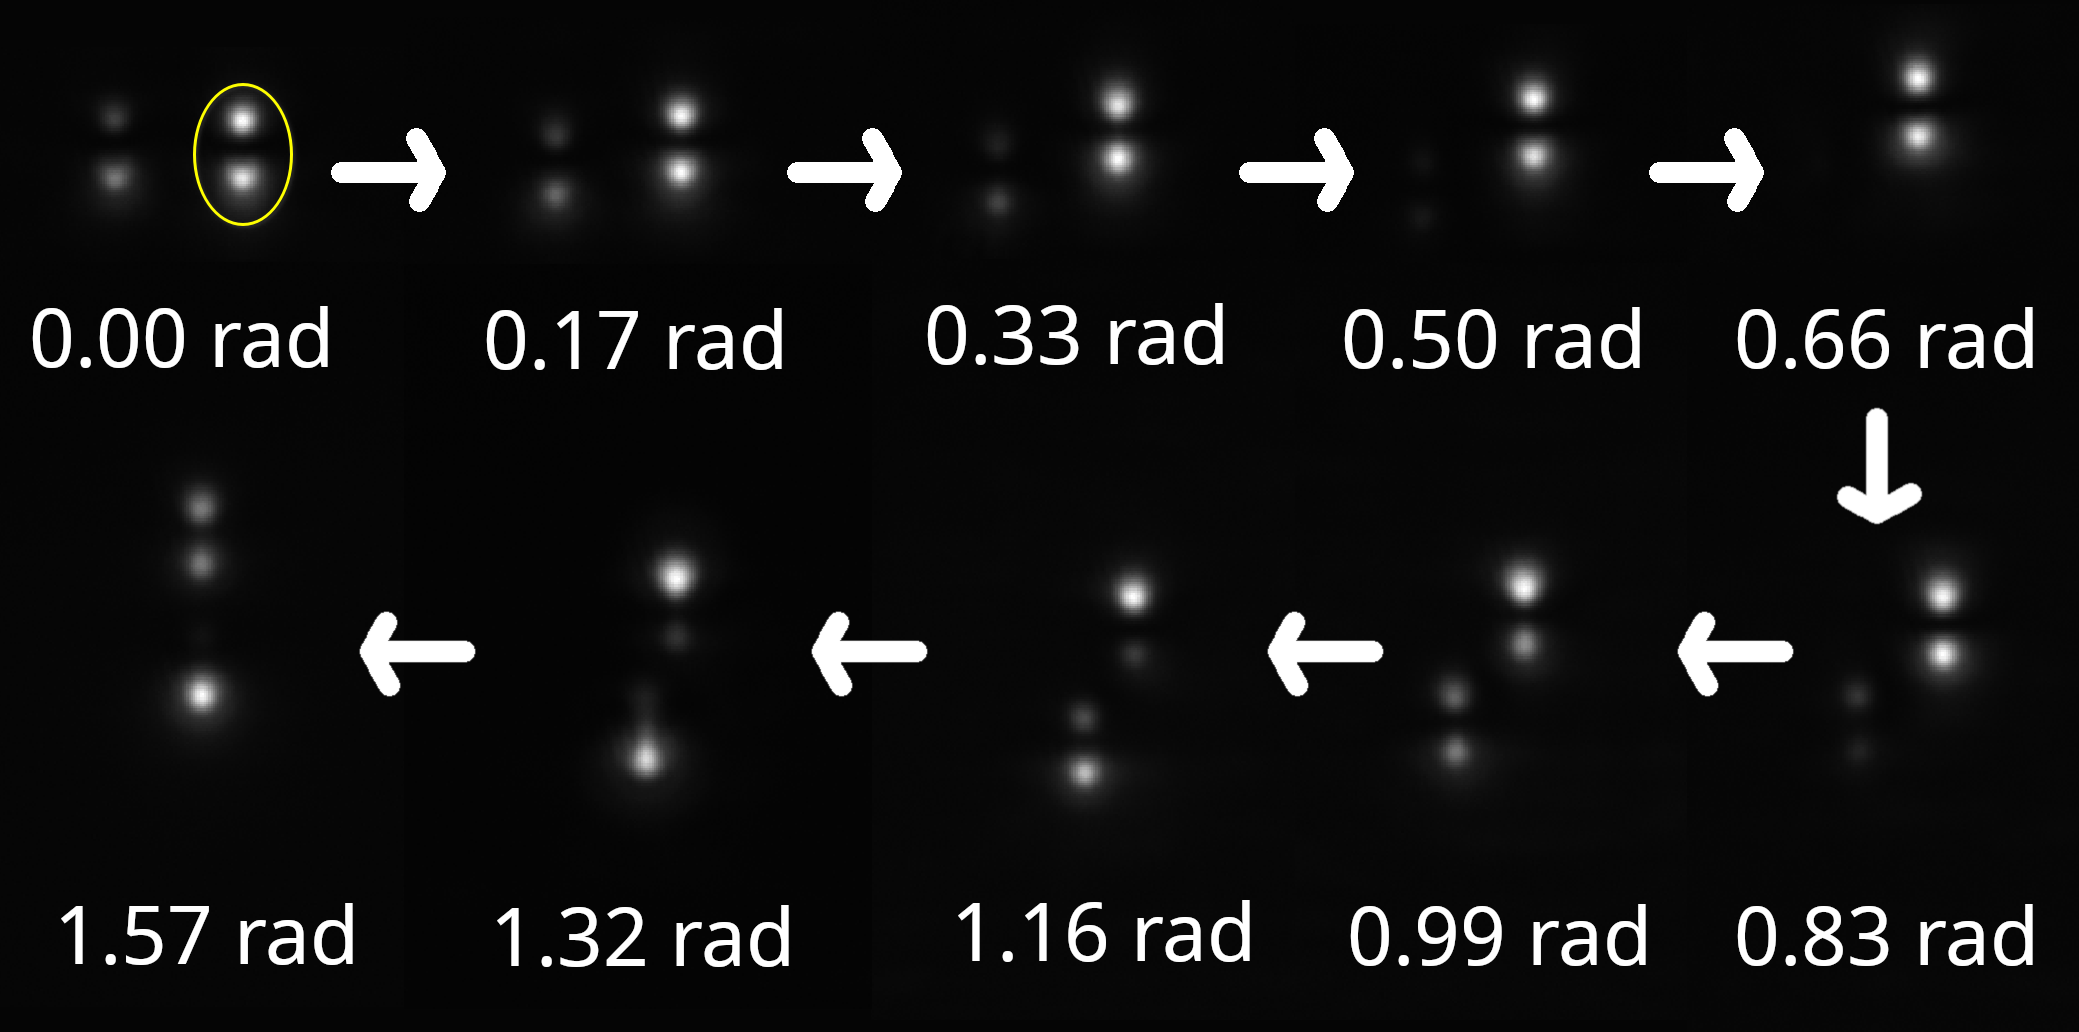
\includegraphics[width=0.7\linewidth]{media/26um_15mm_angles_v2.png}
    \caption[Barrido angular experimental]{Barrido angular experimental para una distancia de propagación de 15 mm. Se observa el efecto del ángulo mágico entre 0.50 y 0.66 rad. \label{fig:angulobarrido}}
\end{figure} \vspace{-2ex} Se analizaron las imágenes siguiendo el método descrito en la Sección \ref{sec:analimag}. Posteriormente, mediante la ecuación (\ref{eqn:coupling-simp}) para el acoplamiento dinámico, se caracterizó su comportamiento en función del ángulo $\theta$ (medido desde la horizontal) para una separación fija de 25 $\mu$m. El signo negativo se introdujo para garantizar la continuidad de la tendencia de los datos, como muestra la Figura \ref{fig:invisibility-coup}.
\begin{figure}[H]
    \centering
    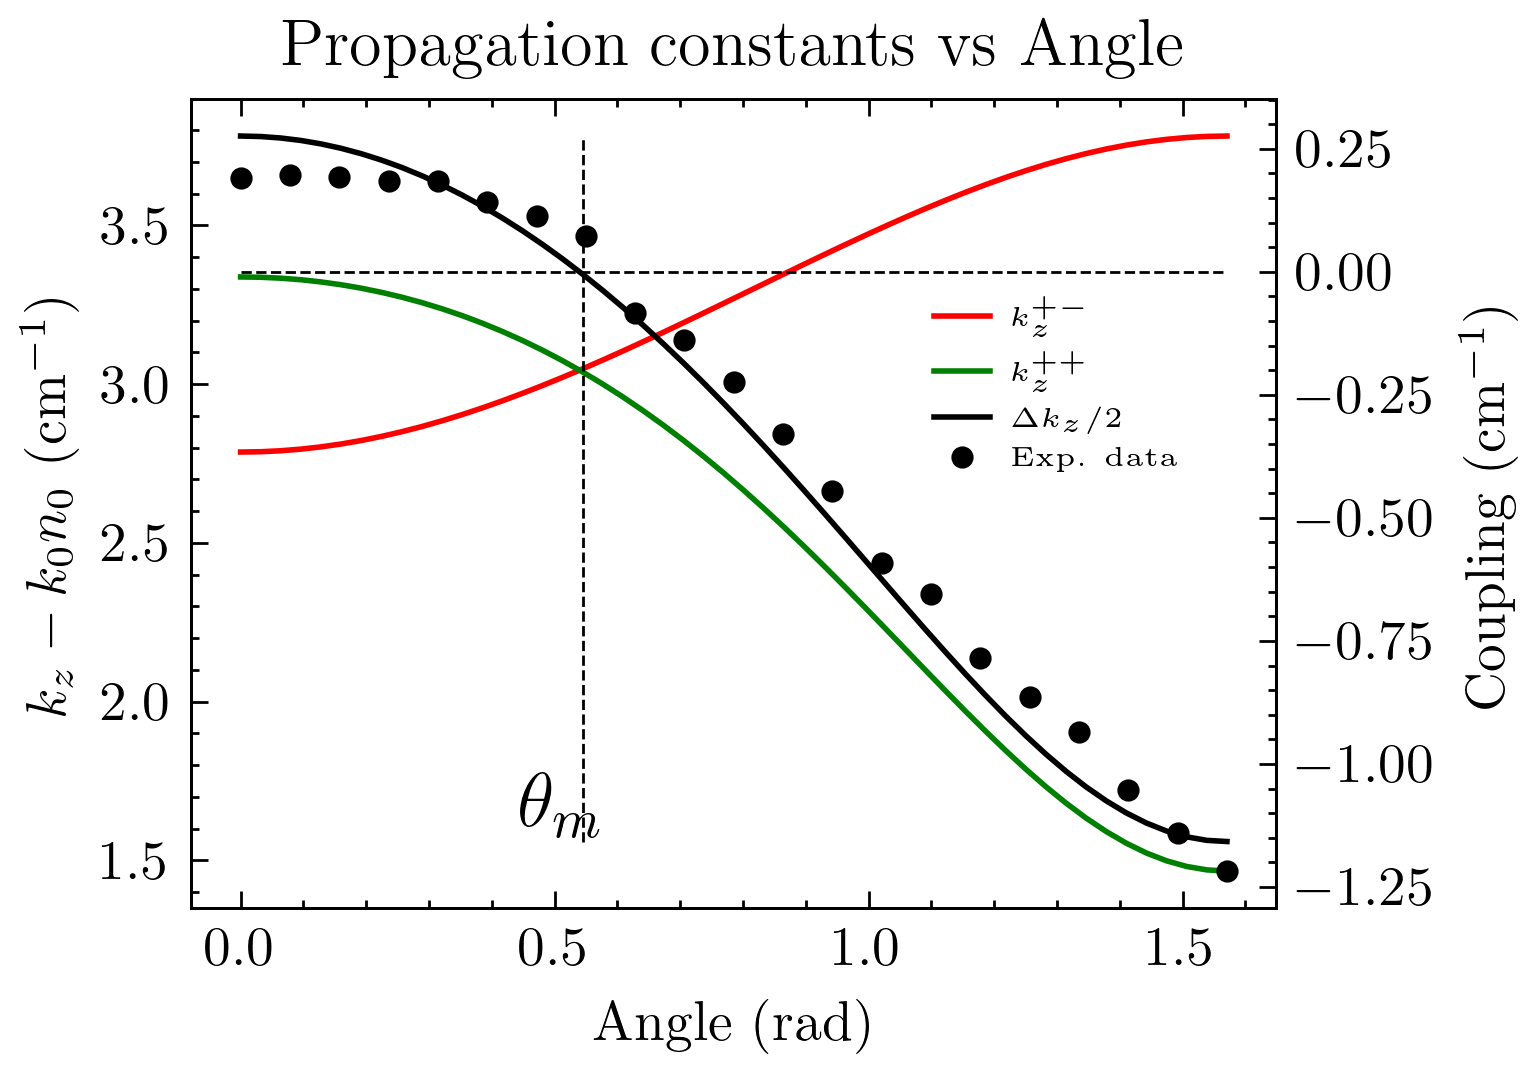
\includegraphics[width=0.6\linewidth]{codigo/eigenvalues_vs_angle.png}
    \caption[Constantes de propagación y acoplamientos angulares para modos P]{Constantes de propagación y acoplamientos en función del ángulo para modos $p_y$, calculados numéricamente mediante EME. Los resultados se comparan con los datos experimentales extraídos de la Figura \ref{fig:angulobarrido}. \label{fig:invisibility-coup}}
\end{figure} \vspace{-2ex}
\section{Redes tipo panal de abeja}
La red tipo panal de abeja, conocida por ser la estructura subyacente del grafeno, presenta propiedades relevantes para esta tesis, particularmente en sus bandas de Bloch: ambas son dispersivas y exhiben un punto de Dirac \citep{honeycombdirac}. Una vez determinados los parámetros de fabricación en la sección anterior, se estudió el mismo efecto en una red tipo panal de abeja manteniendo constante la distancia entre sitios mientras se variaba el ángulo (Figura \ref{fig:HCLBW}).
\begin{figure}[H]
	\centering
	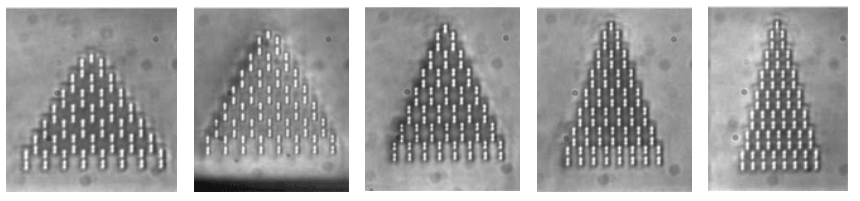
\includegraphics[width=\linewidth]{media/honeycomb_lattices_bw.png}
	\caption[Micrografías de redes fotónicas tipo panal de abeja para modos P]{Micrografías de redes fotónicas tipo panal de abeja para modos $p_y$ bajo iluminación con luz blanca. \label{fig:HCLBW}}
\end{figure} \vspace{-3ex} Un modelo de primeros vecinos consideraría únicamente el acoplamiento vertical $\varkappa_\sigma$ y el acoplamiento angular $\varkappa_\theta$. Sin embargo, la descripción precisa de los datos experimentales requiere incluir acoplamientos hasta terceros vecinos, así como correcciones por no ortogonalidad. La Figura~\ref{fig:honeycombmodel} muestra un esquema del modelo completo. El Hamiltoniano del sistema se expresa como:
\begin{equation}
	\hat{H}_\Sigma = \hat{H}_{NN} + \hat{H}_{NNN} + \hat{H}_{NNNN},
\end{equation}
donde $\hat{H}_{NN}$, $\hat{H}_{NNN}$ y $\hat{H}_{NNNN}$ contienen los acoplamientos a primeros vecinos ($\varkappa_\sigma$ y $\varkappa_\theta$), segundos vecinos ($t_\pi$ y $t_{\theta 2}$), y terceros vecinos ($t_{\theta 1}$ y $t_{\theta 3}$), respectivamente (ver Figura \ref{fig:honeycombmodel}).

\begin{figure}[H]
	\centering
	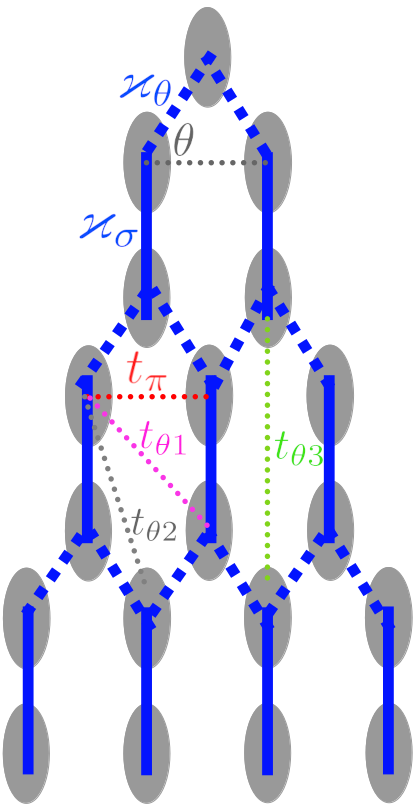
\includegraphics[width=0.25\linewidth]{media/honeycomb-lattice.png}
	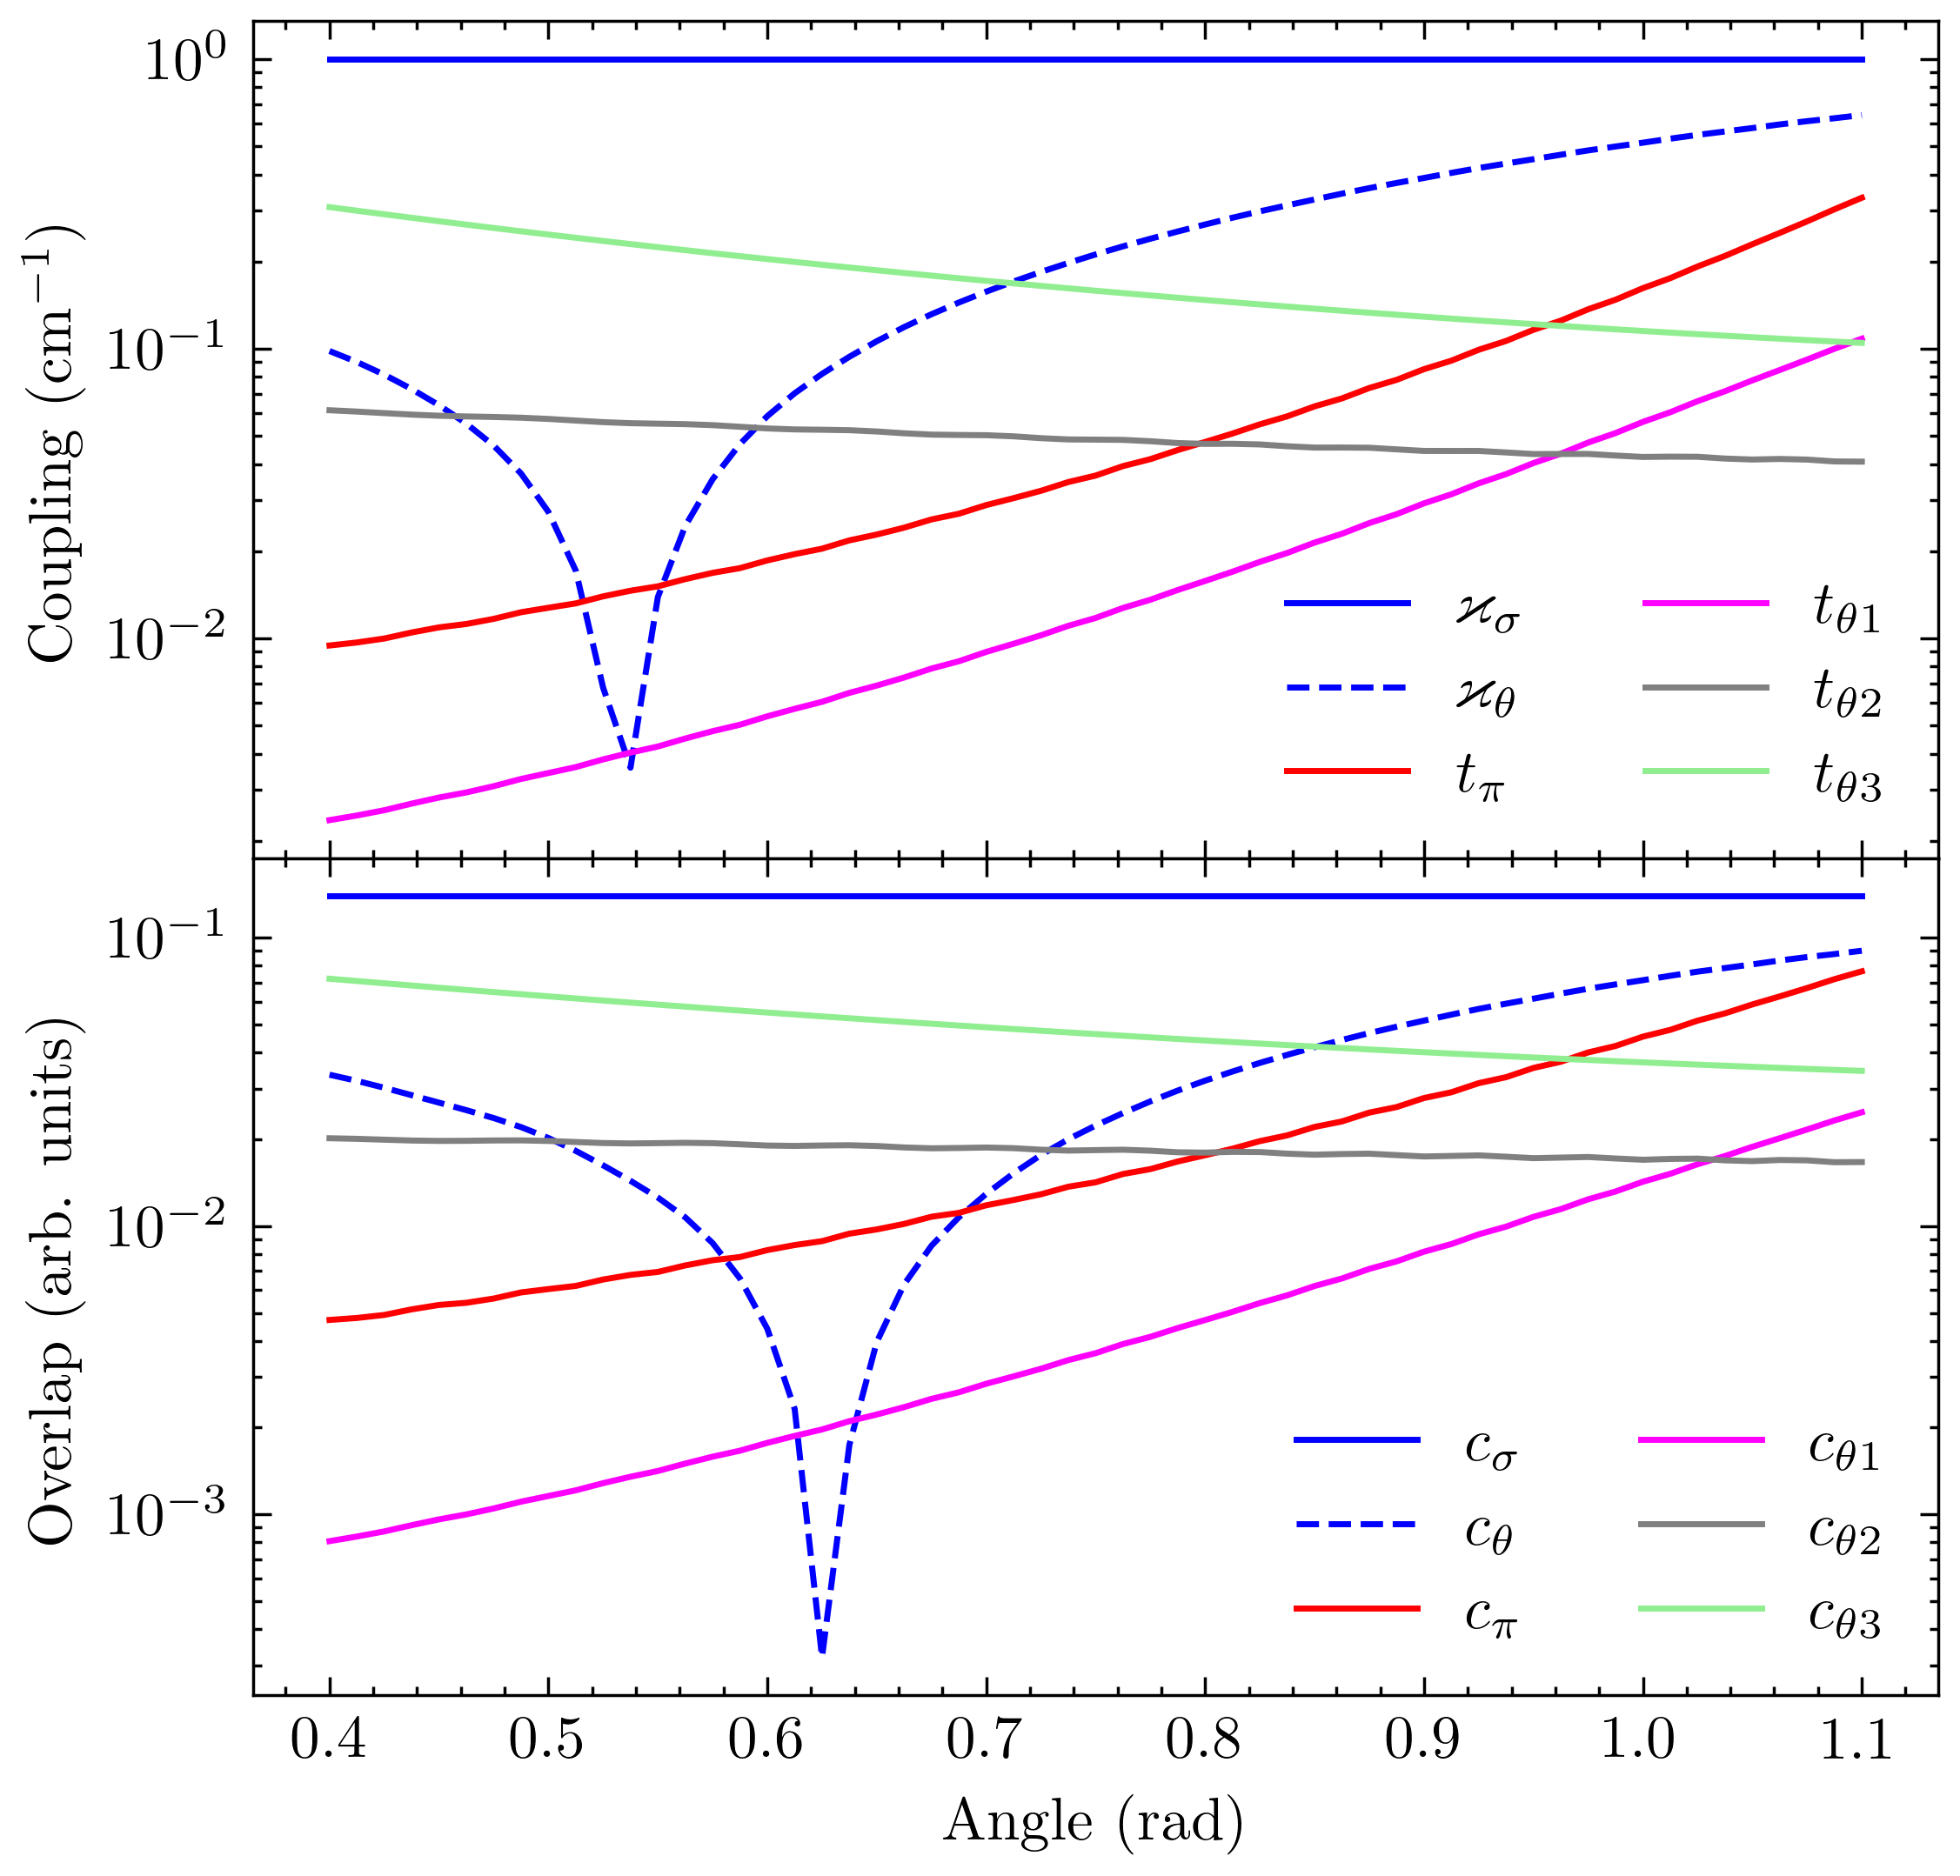
\includegraphics[width=0.55\linewidth]{codigo/NNNN_overlap_vs_angle.png}
	\caption[Modelo de panal de abeja para modos $p_y$ con acoplamientos hasta terceros vecinos]{\textbf{Izquierda:} Esquema del modelo de panal de abeja para modos $p_y$ con acoplamientos hasta terceros vecinos. \textbf{Derecha:} (Arriba) Valores absolutos de los acoplamientos en función del ángulo $\theta$. (Abajo) Integrales de solapamiento normalizadas en función del ángulo $\theta$.\label{fig:honeycombmodel}}
\end{figure} \vspace{-3ex} Además, se define la matriz no ortogonal $\hat{c}$ a partir de la matriz $\hat{P}$ [ecuación~(\ref{eqn:CMTnum})] como $c_{ij} = P_{ij}/I$, donde $I = P_{ii}$ es la intensidad del modo $p_y$, de modo que los elementos diagonales de $\hat{c}$ sean iguales a 1. De manera similar a los acoplamientos, en la Figura \ref{fig:honeycombmodel} se grafica la magnitud de los solapes en función del ángulo.

El Hamiltoniano no hermítico $\hat{H}_\Sigma' \equiv \hat{c}^{-1} \hat{H}_\Sigma$ describe la dinámica de la red e incorpora tanto efectos no ortogonales como acoplamientos de largo alcance. En la Figura \ref{fig:honeycomb-spectra} se muestra el espectro en función del ángulo $\theta$. Se distinguen principalmente dos regiones: una para ángulos $0.4 < \theta < 0.7$, en la que los autovalores se agrupan en tres bandas cuasiplanas, y otra para ángulos $0.7 < \theta < 1.1$, en la que la brecha disminuye en magnitud y, por tanto, se incrementa el transporte en la red. Se calcula el grado de participación inverso (IPR, por sus siglas en inglés) de cada autoestado como $\text{IPR} = \sum_i I_i^2/(\sum_i I_i)^2$. Esto permite la descripción adecuada de los datos experimentales mostrados en el panel derecho de la Figura \ref{fig:honeycomb-spectra}.
\begin{figure}[H]
	\centering
	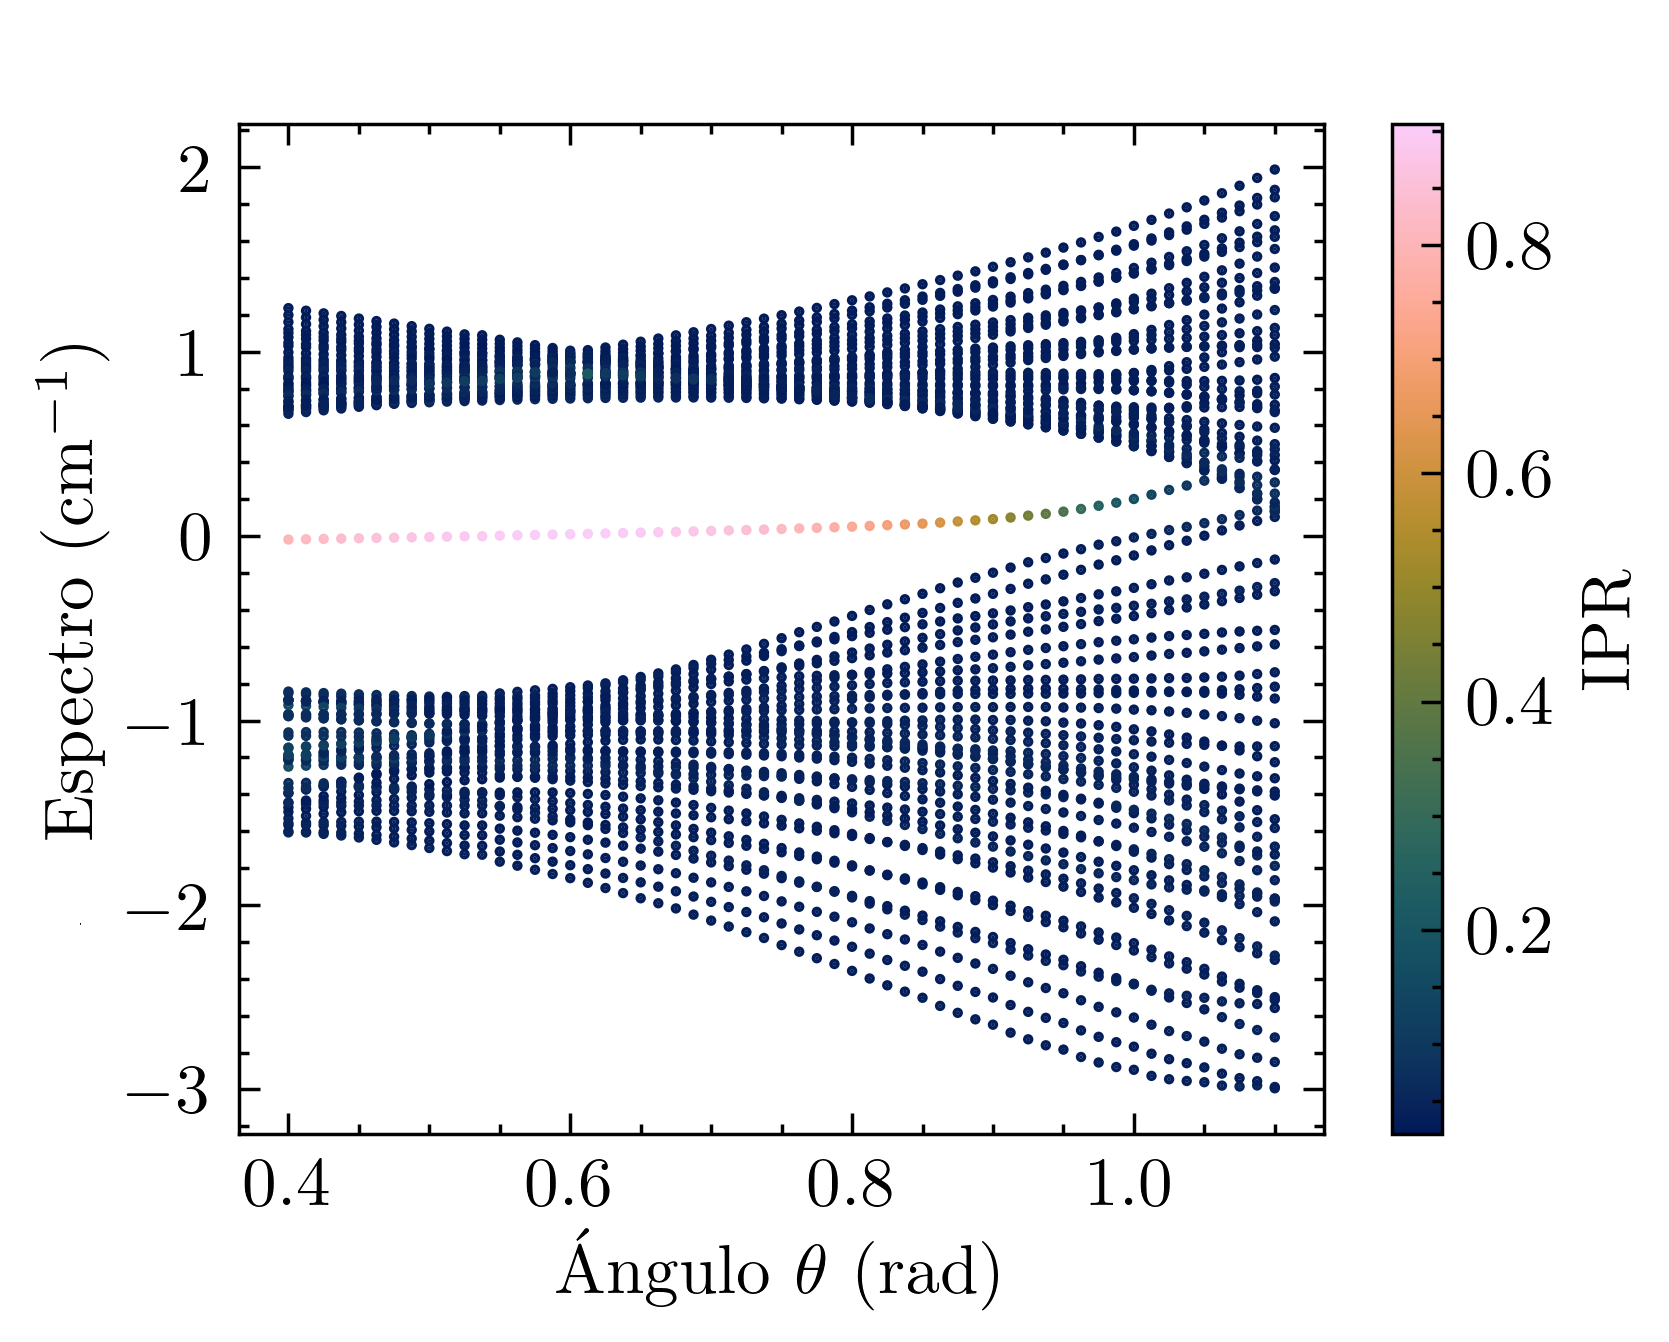
\includegraphics[width=0.45\linewidth]{codigo/honeycomb_eigenvalues_vs_angle.png}
	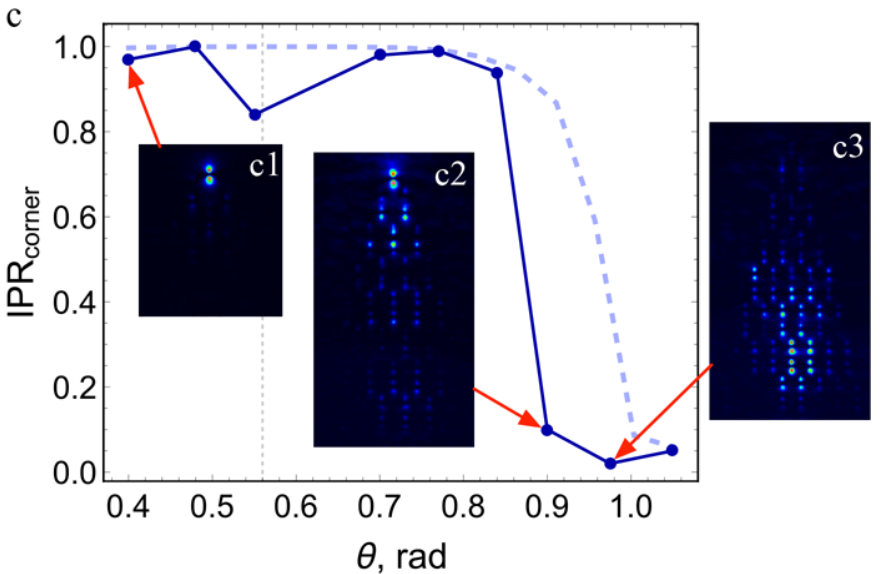
\includegraphics[width=0.5\linewidth]{media/ipr-corner-exp.png}
	\caption[Espectro de la red de panal de abeja de modos $p_y$ en función del ángulo]{\textbf{Izquierda:} Espectro de la matriz $\hat{H}_\Sigma'$ en función del ángulo. Cada punto se colorea según su grado de participación inverso (IPR). \textbf{Derecha:} Grado de participación inverso para la excitación del sitio de esquina en función del ángulo $\theta$.\label{fig:honeycomb-spectra}}
\end{figure} \vspace{-3ex}
La fuerte localización observada al excitar el sitio de esquina se explica porque la proyección de la condición inicial sobre los autoestados corresponde mayoritariamente al autoestado de autovalor nulo. La existencia de este autoestado se debe a la topología que presenta el Hamiltoniano $\hat{H}_\Sigma'$ en el espacio recíproco o de Bloch. Si bien es posible calcular la polarización de bulto mediante bucles de Wilson y determinar que su valor está cuantizado como $\mathbf{P} = (0.5, 0.5)$, resulta más ilustrativo notar que la red puede descomponerse en cadenas cuasi-SSH (ver Figura \ref{fig:cuasi-ssh}). En ambos esquemas, la cuantización es consecuencia de la simetría de inversión presente en la red. 

\begin{figure}[H]
	\centering
	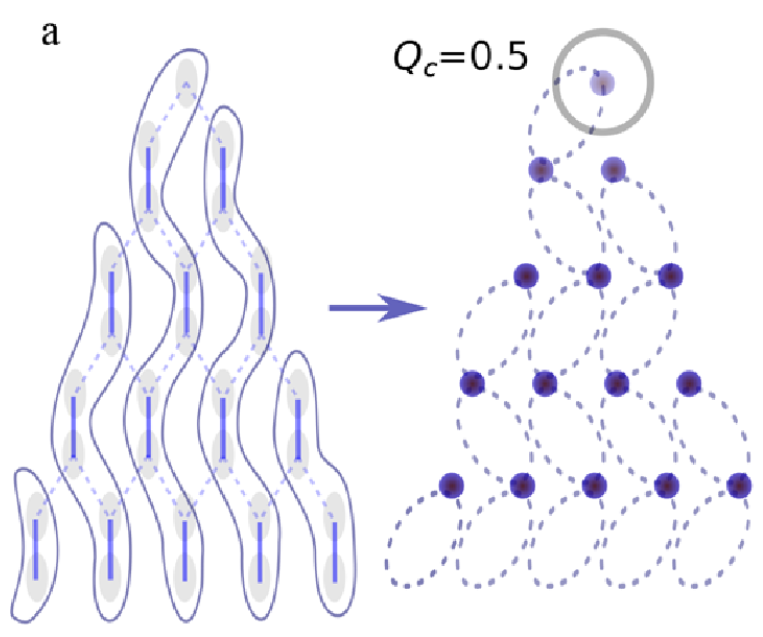
\includegraphics[width=0.5\linewidth]{media/cuasi-ssh.png}
	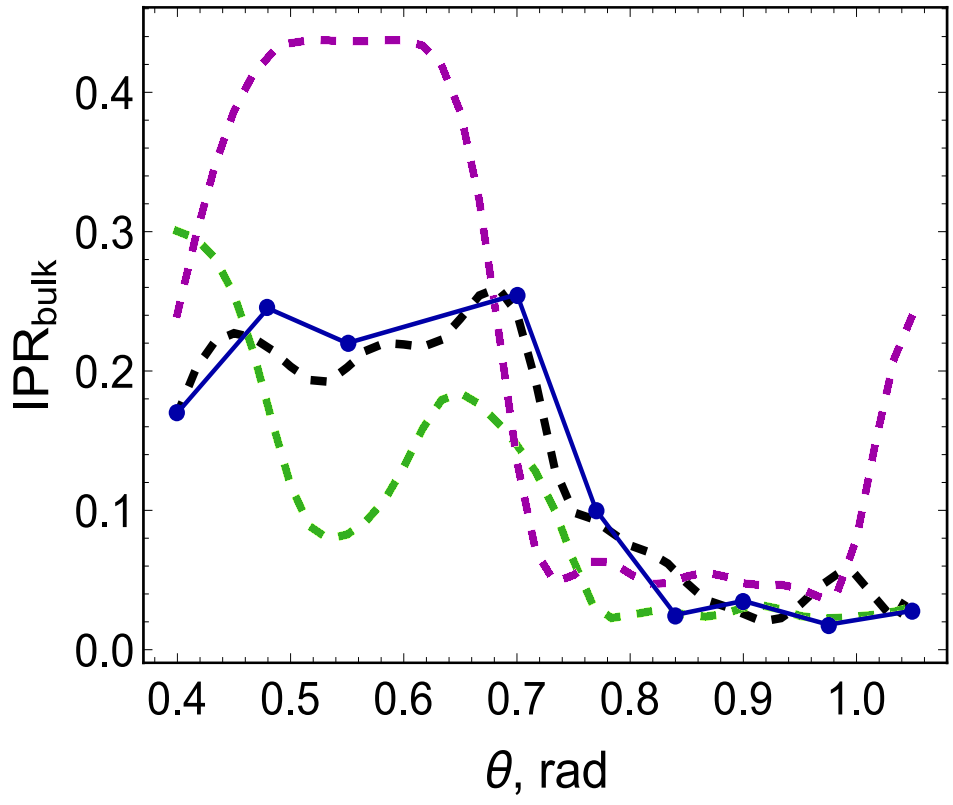
\includegraphics[width=0.45\linewidth]{media/ipr-bulk-exp.png}
	\caption[Descomposición de la red en cadenas cuasi-SSH]{  
		\textbf{Izquierda: }  
		Descomposición de la red en el límite de bandas planas en cadenas SSH de dímeros aislados. \textbf{Derecha: }  IPR para la excitación experimental del sitio central de la red (puntos unidos con líneas para guiar la vista) y simulados numéricamente para tres casos: sin acoplamientos de largo alcance ni correcciones no-ortogonales (curva morada discontinua), con acoplamientos de largo alcance pero sin correcciones no-ortogonales (curva verde discontinua), y con acoplamientos de largo alcance y correcciones no-ortogonales (curva negra discontinua).  \label{fig:cuasi-ssh}}
\end{figure} \vspace{-2ex}
Se estudió experimentalmente la dinámica de bandas planas excitando un único sitio en el bulto de la red para extraer su IPR. Como la excitación inicial en un solo sitio tiene proyecciones no nulas en todas las bandas de Bloch, este experimento magnifica las propiedades dispersivas de las bandas. Así, una propagación casi sin difracción implica una notable planitud de todas las bandas, pues las propiedades de bulto de una red se manifiestan más claramente cuando se excita un sitio central. Un sistema con todas sus bandas planas no exhibiría transporte en la red, limitándose la dinámica únicamente a dímeros efectivos.

Los datos analizados revelan dos regímenes distintos: para redes con $0.4 < \theta < 0.8$ (cercanas al ángulo de invisibilidad) se observa un buen efecto de confinamiento (\emph{caging}). Sin embargo, ángulos mayores ($\theta > 0.8$) favorecen una difracción significativa del campo, resultando en una deslocalización a la salida. Estos resultados experimentales (puntos en Figura \ref{fig:cuasi-ssh}) concuerdan con los cálculos teóricos (línea discontinua). Contrario a lo esperado, los acoplamientos de largo alcance y las correcciones por no ortogonalidad no degradan la dinámica de bandas planas cerca del ángulo de invisibilidad, sino que se complementan. Los valores máximos de IPR ($0.20$-$0.25$) para el estado dímero después de tres ciclos de confinamiento Aharonov-Bohm indican una localización comparable con propuestas ópticas unidimensionales con todas sus bandas planas (ABF). 
\chapter{Moléculas Fotónicas}

La técnica de escritura de guías de onda descrita en el capítulo \ref{cap:fs} está restringida por la forma alargada y elíptica del tren de pulsos láser que se enfoca, lo que en consecuencia constriñe los acoplamientos interorbitales posibles \citep{interorbital}. Una posibilidad para añadir grados de libertad es fabricar dos guías de onda lo suficientemente cercanas entre sí de manera de hibridizar sus modos guiados, de manera análoga al principio físico que rige a las moléculas. Es por ello que en este capítulo se usará el concepto de moléculas fotonicas \citep{molecules}, y su aplicación para el estudio experimental de una red fotónica que presenta una doble transición de fase topológica \citep{SPSSH}.

\section{Autoestados del acoplador fotónico para distancias de separación arbitrarias}

Como se adelantó en la sección \ref{cap:maxwell}, la teoría de modos acoplados es una buena descripción de los sistemas fotónicos en estudio siempre que la distancia de separación entre guías de onda sea superior a 15 $\mu$m, pues la constante de acoplamiento tiene un comportamiento exponencial decreciente. Más allá del régimen discreto, se hace necesario descibir el sistema como una sola macroguía. Una herramienta numérica que es agnóstica entre ambos regímenes es la de Expansión en Modos Normales, detallada en la sección \ref{cap:eme}. Es por ello que se simula un par de guías de onda a distintas distancias para determinar el comportamiento de sus autoestados. 

\begin{figure}[H]
	\centering
	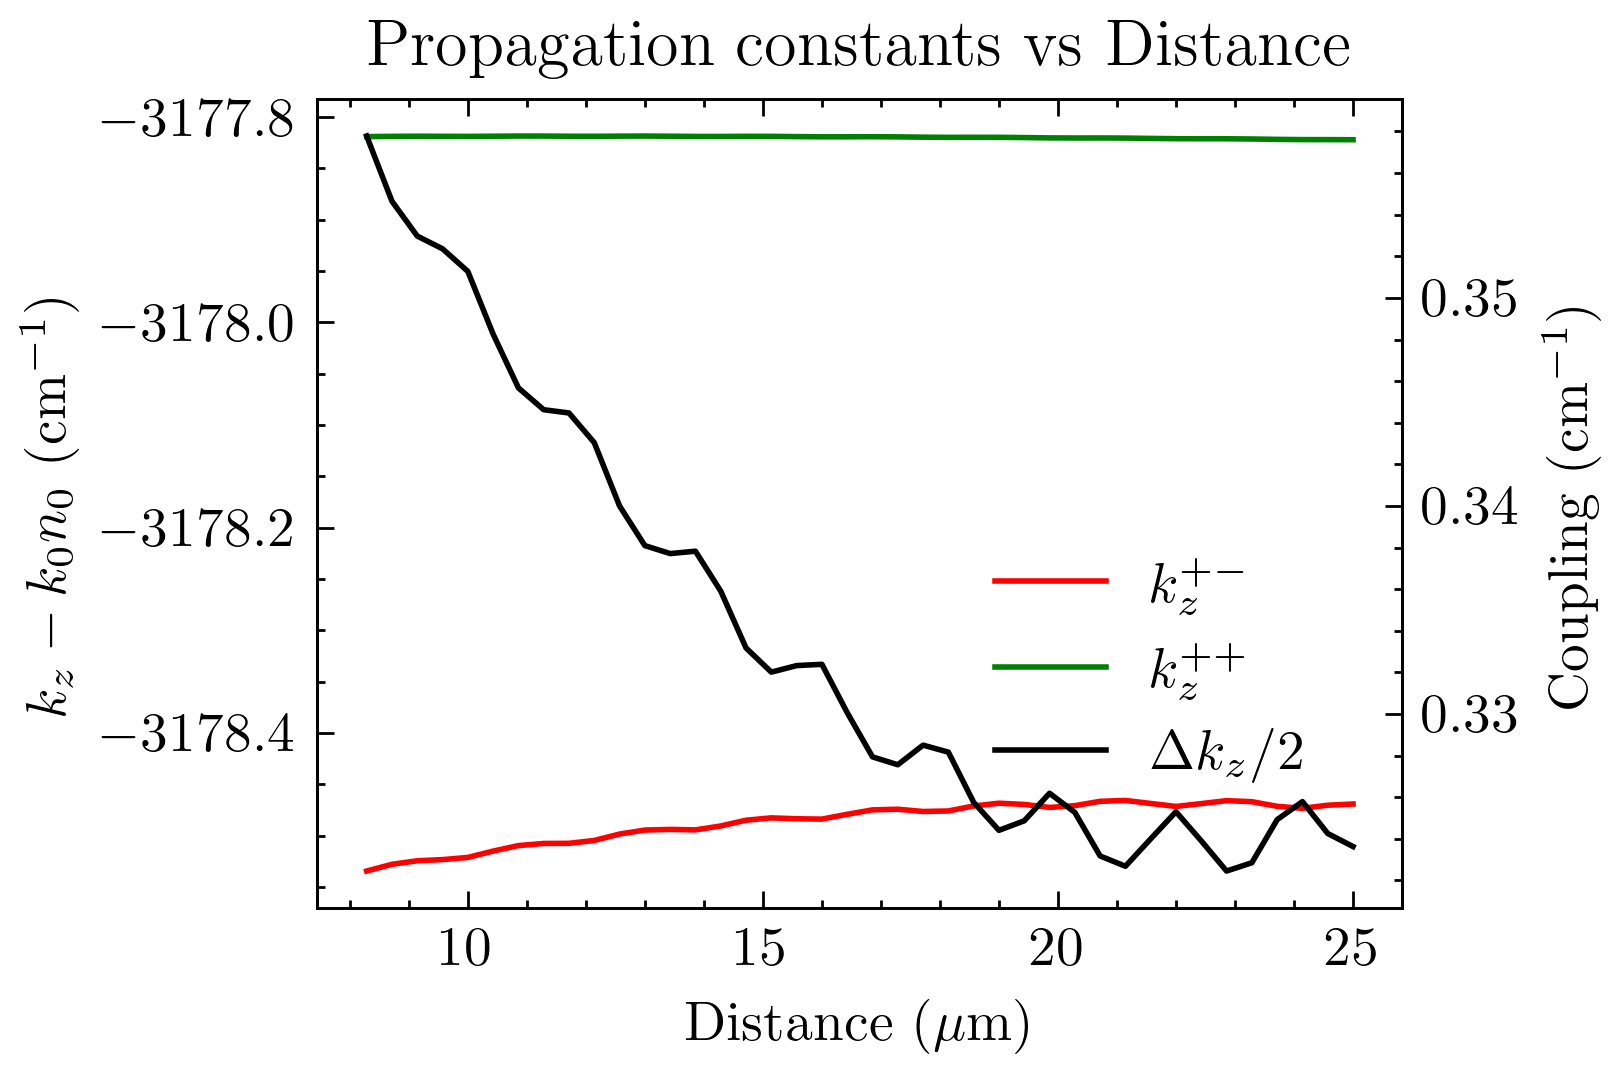
\includegraphics[width=0.7\linewidth]{codigo/dimol2/eigenvalues_vs_angle.png}
	\caption[Constantes de propagación y acoplamientos angulares para modos fundamentales]{Constantes de propagación y acoplamientos en función del ángulo para modos fundamentales, calculados numéricamente mediante EME. \label{fig:molecule-coup}}
\end{figure}

\section{Moléculas Fotónicas en Red SP-SSH}

Para la implementación experimental (sección \ref{cap:fs}) de una red que presente acoplamiento SP \citep{interorbital, SPSSH}, se utilizaron los dipolos horizontales de la sección anterior, obtenidos mediante moléculas fotónicas. Un preciso sintonizado de las constantes de propagación de los modos $s$ y $p$ permitió considerar un grado de libertad análogo al del espín del electrón (\textit{pseudoespín}). El Hamiltoniano $H$ de esta red \citep{SPSSH,toporusos}  es el siguiente

\begin{align*}
	H &= \sum_n \left[\frac{\delta\beta}{2} \left( b^*_{n, 1} b_{n, 1} - a^*_{n, 1} a_{n, 1} + b^*_{n, 2} b_{n, 2} - a^*_{n, 2} a_{n, 2} \right) +k_{ss, 2}a^*_{n, 2} a_{n, 1} -k_{pp, 2}b^*_{n, 2} b_{n, 1} \right. 
	\\	
	&+ k_{ss, 1} \left( a_{n-1, 2}^*a_{n, 1} + a_{n+1, 2}^*a_{n, 2} \right) - k_{pp, 1} \left( b_{n-1, 2}^*b_{n, 1} + b_{n+1, 2}^*b_{n, 2} \right) + k_{sp, 2} \left( a_{n, 2}^* b_{n, 1} - b_{n, 2}^* a_{n, 1} \right)
	\\
	&+ \left. k_{sp, 1} \left( a_{n-1, 2}^* b_{n, 1} - b_{n-1, 2}^* a_{n, 1} + a_{n+1, 1}^*b_{n, 2} - b_{n+1, 1}^* a_{n, 2} \right) \right] + c.c.
\end{align*}

\begin{figure}[H]
\centering
	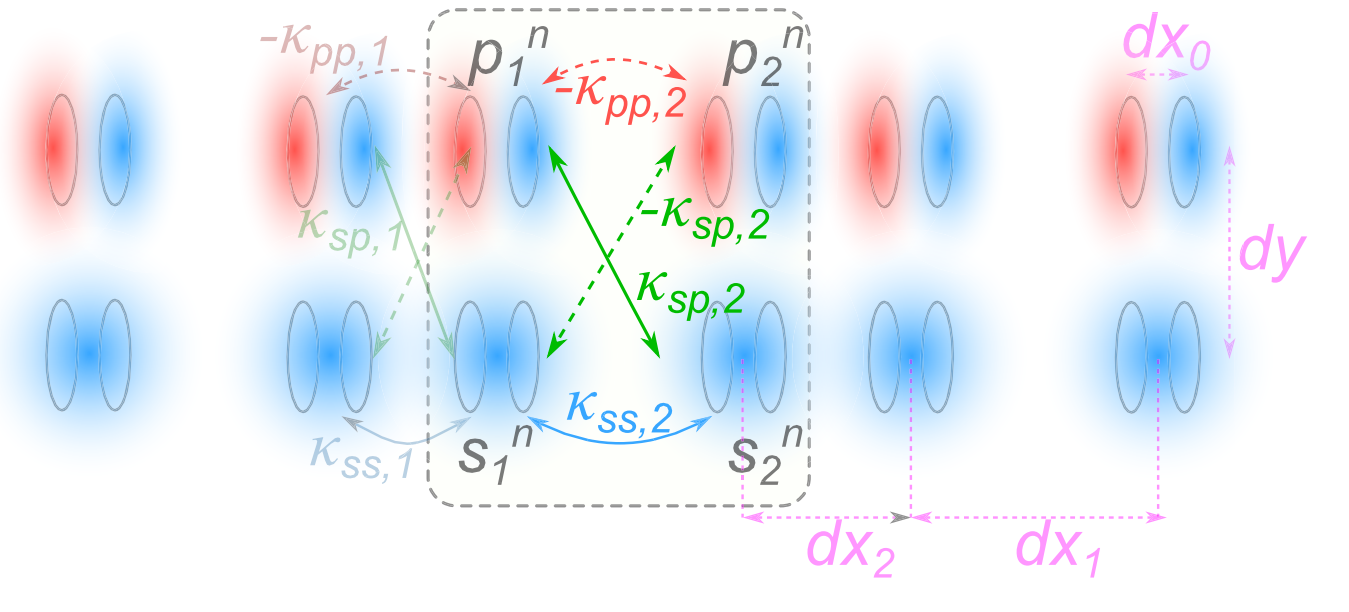
\includegraphics[width=0.7\linewidth]{media/ssh_sp_model}
	\caption{Esquema de la red SP-SSH.}
\end{figure}
\chapter{Haces Con Momentum Orbital Angular}





\chapter{Conclusiones}

\lipsum[130-132]
\begin{figure}
	\centering
	
\includegraphics[scale=.2]{imagenes/fcfm.pdf}
	\caption{Logo de la Facultad}
	\label{logofcfm}
\end{figure}

\lipsum[133-134]

\begin{table}
	\centering
	\caption{Tabla 1}
	\label{tabla:1}
	\begin{tabular}{|c|c|r|}
		\hline
		\textbf{Campo 1} & \textbf{Campo 2} & \textbf{Num} \\\hline
		Valor 1a & Valor 2a & 3\\
		Valor 1b & Valor 2b & 3\\
		\hline
	\end{tabular}

\end{table}

\lipsum[135]


% ver https://www.overleaf.com/learn/latex/Glossaries
% \input{glosario.tex} % opcional

%\nocite{*}
\bibliographystyle{unsrtnat}
\bibliography{citations}

% opcional ...
\renewcommand\appendixname{Anexo}
\begin{appendices}
\section{Ortogonalidad de los modos normales \label{sec:orto}}

La ortogonalidad de los modos normales $\textbf{E}_\nu^\perp$ puede demostrarse utilizando el convenio de Einstein en la ecuación (\ref{eqn:eigenfield}) para simplificar la notación:
\begin{equation}
	T_{ij} E^\nu_j = \beta_\nu^2 E^\nu_i, \label{eqn:eigentensorial}
\end{equation}
donde el operador $T_{ij}$ actúa como $T_{ij}E_j \equiv \delta_{ij}\left(\nabla_\perp^2 + k_0^2n^2\right)E_j + \partial_i \left(E_j \partial_j\ln(n^2)\right).$

Para demostrar la ortogonalidad de los modos $E_i$, se puede demostrar equivalentemente que $T_{ij}$ es hermítico:
\begin{align}
	\iint \left(T_{ij} E_j^\mu\right)^* E_i^\nu \,dA = \iint \left(E_i^\mu\right)^* \left(T_{ij} E_j^\nu\right) \,dA.
\end{align}
Esta propiedad se sigue de la identidad:
\begin{align*}
	&\left(T_{ji} E_i^\mu\right)^* E_j^\nu - \left(E_i^\mu\right)^* \left(T_{ij} E_j^\nu\right) =  \nabla_\perp \cdot \left[E_i^\nu \nabla_\perp \left(E_i^\mu\right)^* - \left(E_i^\mu\right)^* \nabla_\perp E_i^\nu\right]  + \left[E^\nu_j \partial_j \left(E_i^\mu\right)^* - \left(E_j^\mu\right)^* \partial_j E_i^\nu\right] \partial_i \ln(n^2).
\end{align*}
Al integrar sobre el plano transversal el término de divergencia se anula para modos guiados (que decaen en el infinito), pero el segundo término desaparece sólo si $\nabla n^2 = \textbf{0}$. Es decir, el operador $T_{ij}$ sólo es Hermítico en la condición de guiaje débil.

El sistema completo es hermítico, como se demuestra partiendo de la ecuación (\ref{eqn:rotordoble}):
\begin{align*}
	\iiint_V \left(\nabla\times\nabla\times\textbf{E}^\nu\right) \cdot \left(\textbf{E}^\mu\right)^* dV &= \iiint_V n^2\frac{\omega_\nu^2}{c^2} \textbf{E}^\nu \cdot \left(\textbf{E}^\mu\right)^* dV \\
	\iiint_V \left[\nabla\times\nabla\times\left(\textbf{E}^\mu\right)^*\right] \cdot \textbf{E}^\nu dV &= \iiint_V n^2 \frac{\omega_\mu^2}{c^2} \left(\textbf{E}^\mu\right)^* \cdot \textbf{E}^\nu dV
\end{align*}

Restando ambas ecuaciones y aplicando el teorema de divergencia:
\begin{align*}
	\frac{\omega_\nu^2 - \omega_\mu^2}{c^2} \iiint_V n^2 \textbf{E}^\nu \cdot \left(\textbf{E}^\mu\right)^* dV &= \oiint_{\partial V} \left[ \cdots \right] \cdot \hat{\textbf{n}}\,dA \\
	&\xrightarrow{\partial V \to \infty} 0
\end{align*}
Se obtienen así dos posibilidades: o los modos son degenerados ($\omega_\nu^2 = \omega_\mu^2$), o se tiene que $\iiint n^2 \textbf{E}^\nu \cdot \left(\textbf{E}^\mu\right)^* dV = 0$.
\chapter{Código en Python para cálculo de modos normales \label{sec:codigohelmholtz}}

\chapter{Código en C de BPM \label{sec:codigoBPM}}

\lstinputlisting[language=C]{./codigo/rad2dc.c}
\chapter{Código en Python generador de hologramas \label{sec:codigoSLM}}

\end{appendices}
\end{document}